\subsection{Luminosity Scale Factors}
\label{s:lumi_sf}

The MC events listed in Table~\ref{tab:mcSample} are arbitrarily generated.
While comparing distributions obtained using MC events with that of data, 
the former has to be normalised with the integrated luminosity of data.
To achieve this, each MC sample is multiplied by the following luminosity scale 
factor ($SF_{L}$):
\begin{equation}
SF_{L}=\frac{L_{\rm data}}{L_{\rm MC}} = \frac{L_{\rm data}\times\sigma_{\rm MC}}{N_{\rm MC}},
\label{eq:lumiSF}
\end{equation}
where $L_{\rm data} = 35.5$ \fbinv and $N_{\rm MC}$ is the number of 
generated MC events and $\sigma_{\rm MC}$ is the cross section of MC samples.
As listed in Table~\ref{tab:mcSample}, the $SF_{L}$ value is less than 1 for 
most of the background samples except for QCD.
For QCD it is very large compared to other backgrounds owing to less number of 
generated events compared to its cross-section. Simulation of large number of 
QCD events is not feasible because of computing limitations.  

\subsection{Pileup Reweighting}
\label{s:pileup_reweighting}
The pileup distributions in the data and MC are different. To match the MC 
pileup distribution with that of data, MC events are reweighted. Depending on 
the number of primary vertices, each MC event is multiplied by corresponding 
pileup weight. The pileup weights are the ratio of pileup distributions from 
data and MC. The pileup distributions in data and MC samples are calculated as 
follows:
\begin{itemize}
    \item {\bf pileup distribution in data}: The pileup distribution in the data is 
        calculated using the Command (\ref{cmd:pileupCalc}) and shown in 
        Figure~\ref{subfig:dataPileup}.
    \item {\bf pileup distribution in MC}: The pileup distribution in MC are accessed 
        through the $slimmedAddPileupInfo$ tag from $MINIAOD$ datasets for all MC samples. 
        The "in-time" pileup distributions for \ttjets, $W + jets$, and 
        $Z/\gamma + jets$ are shown in Figures~\ref{subfig:mcPileup_tt},~\ref{subfig:mcPileup_wjet},
        and~\ref{subfig:mcPileup_dy}, respectively. Since the pileup distributions
        are campaign dependent, not sample dependent, we see similar distribution for all 
        the MC samples.
\end{itemize}
The pileup weights are calculated using standard \verb|LumiReweighting| tool 
of CMSSW. The pileup weights as shown in Figure~\ref{subfig:ratioPileup_all} are 
normalised ratio of the pileup distribution from data and MC.
\begin{figure}
    \centering  
  \subfigure[True in-time pileup distribution in \ttjets sample.\label{subfig:mcPileup_tt}]
  {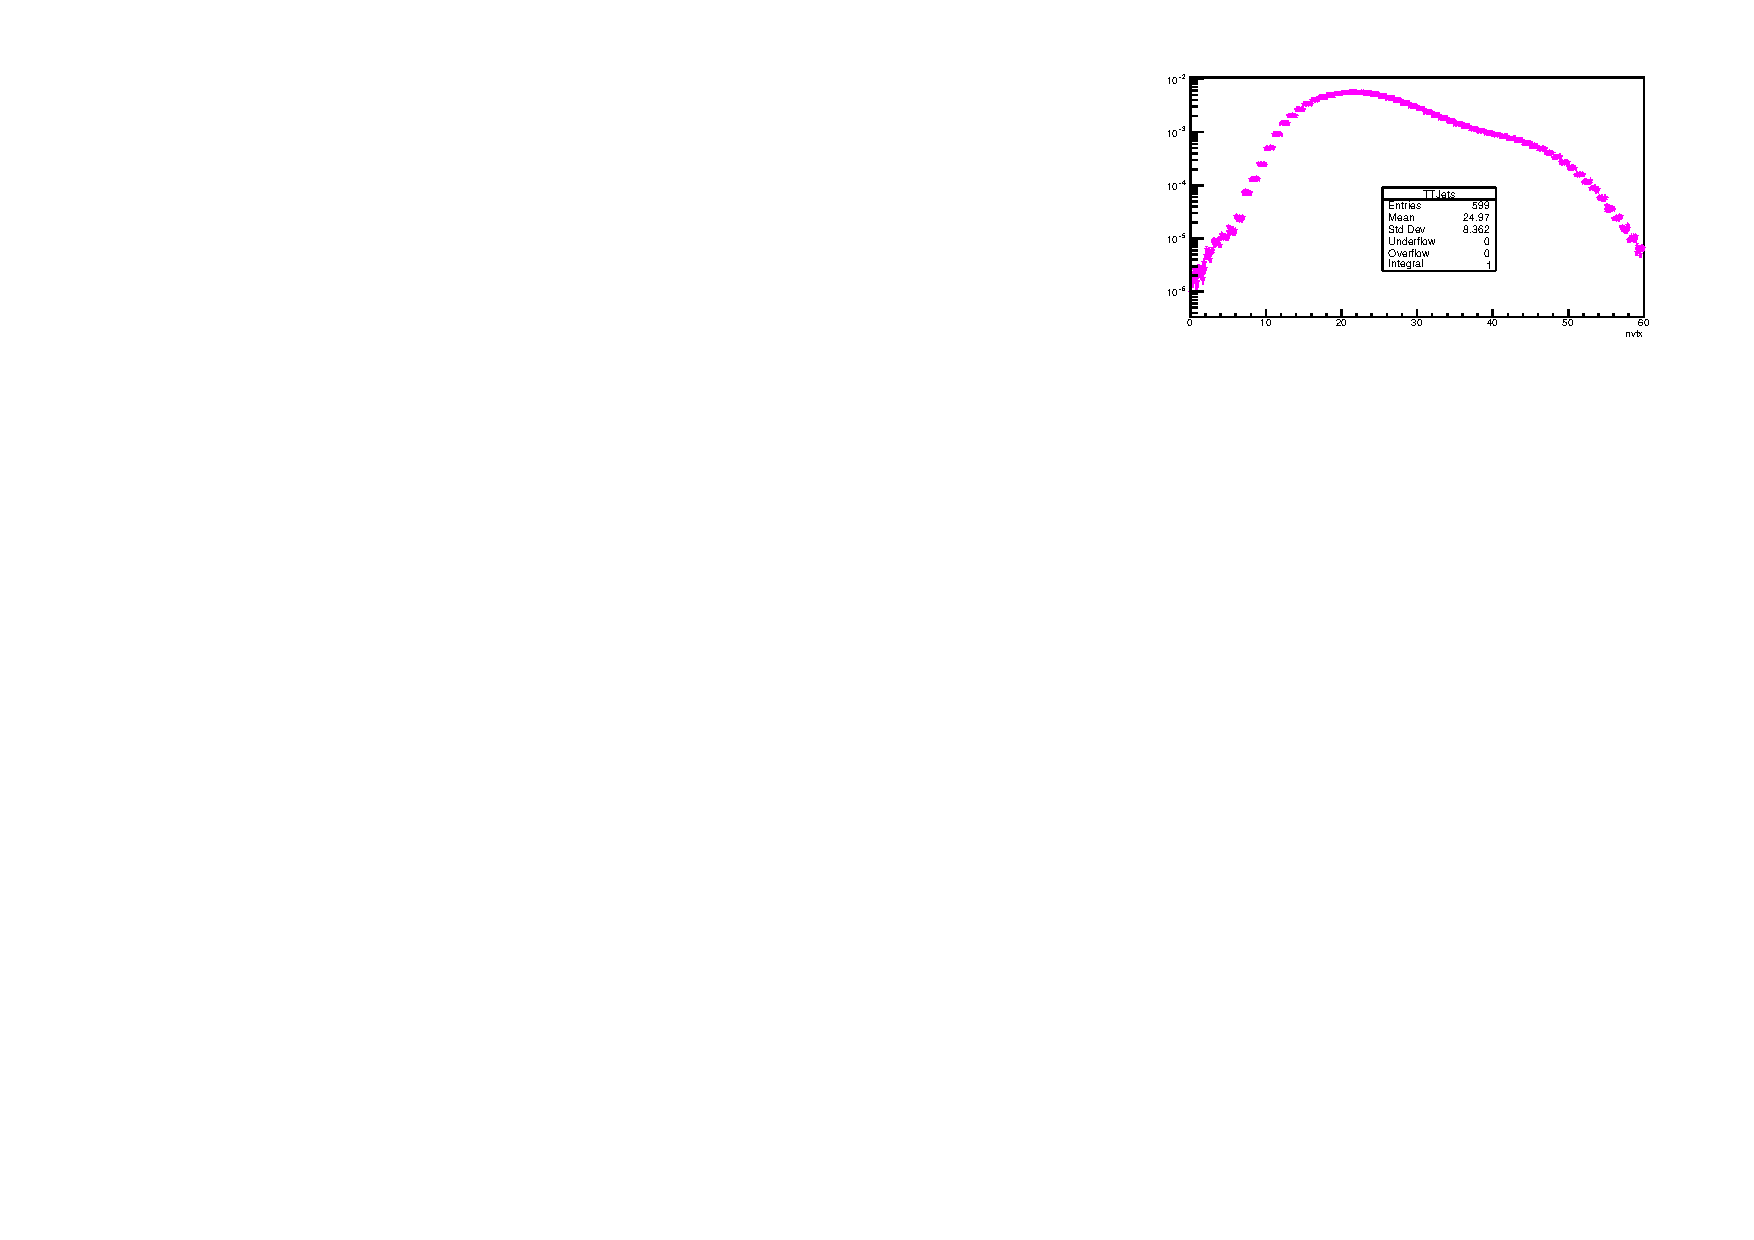
\includegraphics[width=0.49\linewidth]{Image/PU/mcPileup_tt.pdf}}
  \subfigure[True in-time pileup distribution in $W + jets$ sample.\label{subfig:mcPileup_wjet}]
  {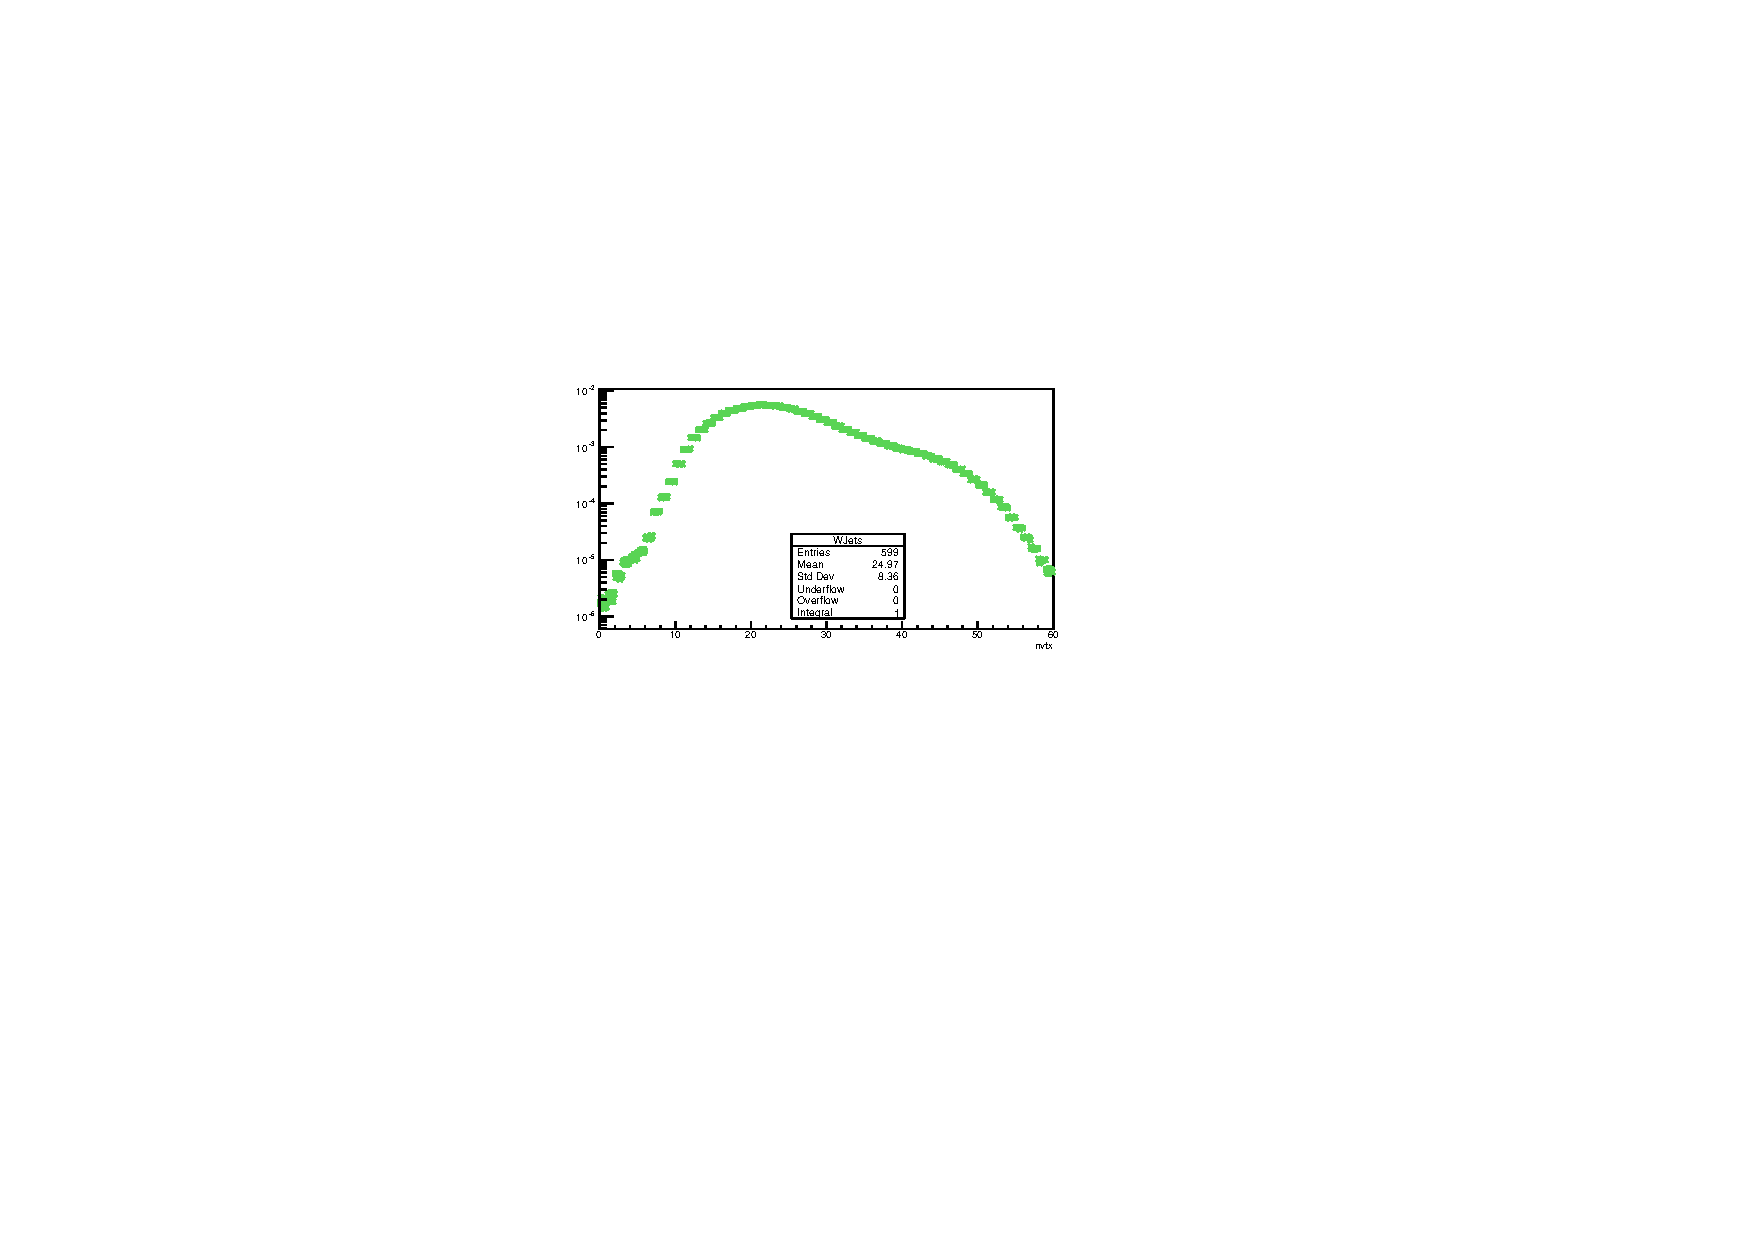
\includegraphics[width=0.49\linewidth]{Image/PU/mcPileup_wjet.pdf}}
  \vfil 
  \subfigure[True in-time pileup distribution in $Z/\gamma + jets$ sample. \label{subfig:mcPileup_dy}]
  {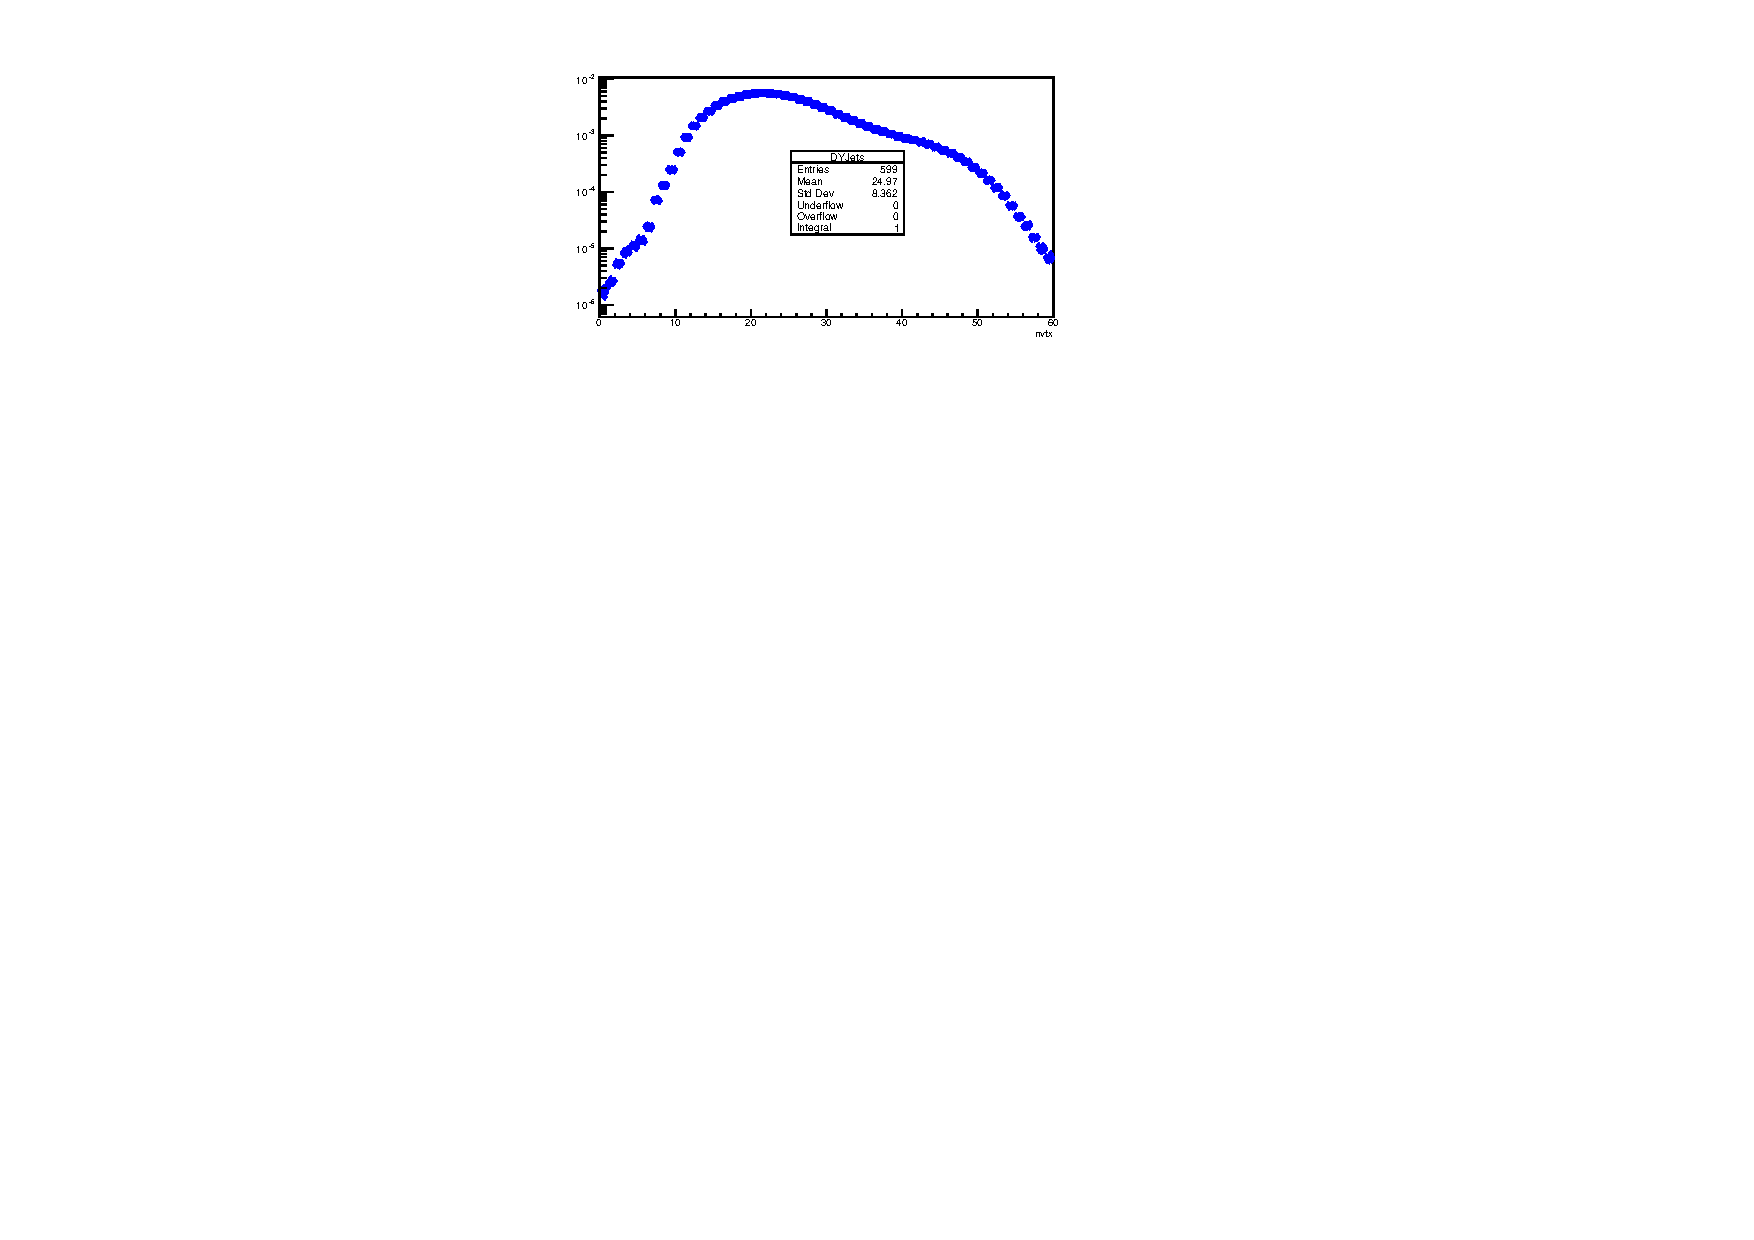
\includegraphics[width=0.49\linewidth]{Image/PU/mcPileup_dy.pdf}}
  \subfigure[True in-time pileup distribution in muon data.\label{subfig:dataPileup}]
  {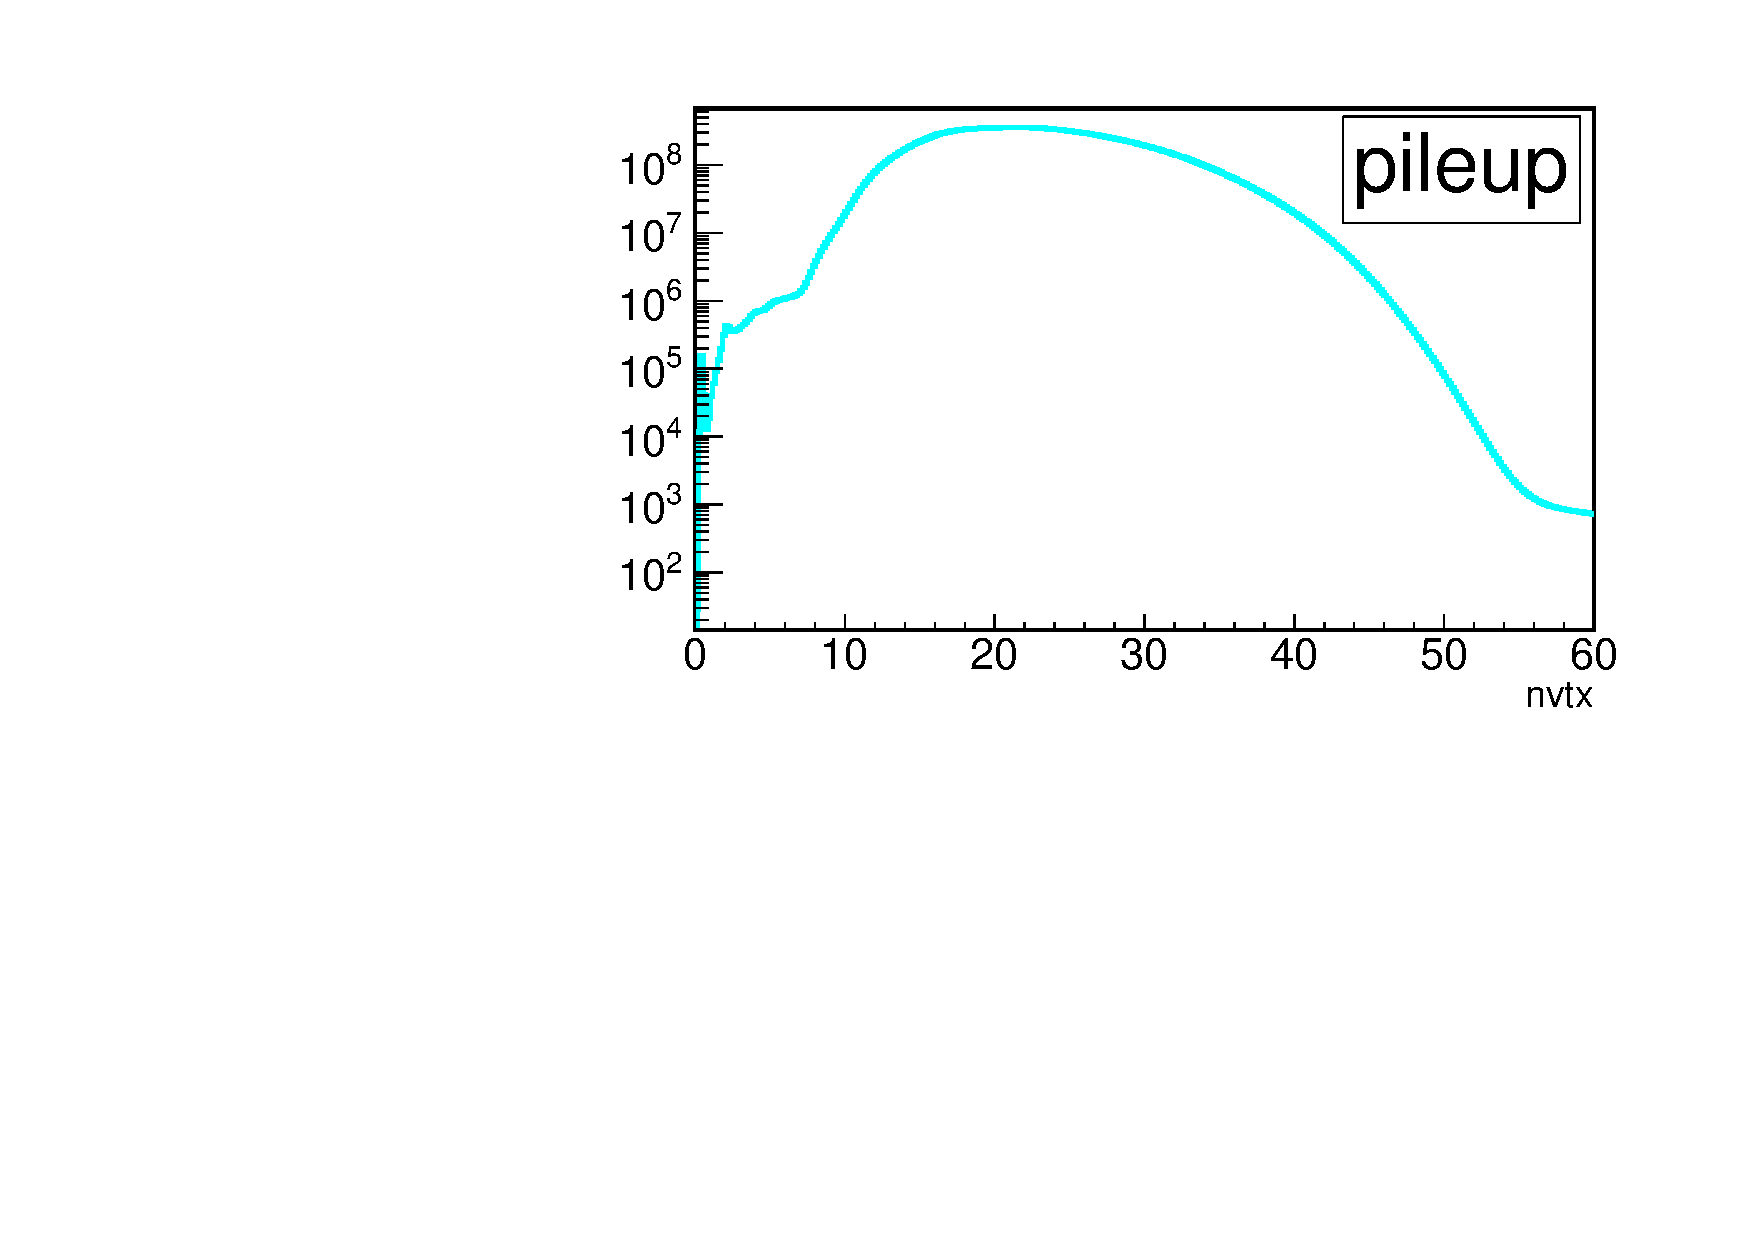
\includegraphics[width=0.50\linewidth]{Image/PU/dataPileup.pdf}}
  \vfil 
  \subfigure[Pileup weight distributions.\label{subfig:ratioPileup_all}]
  {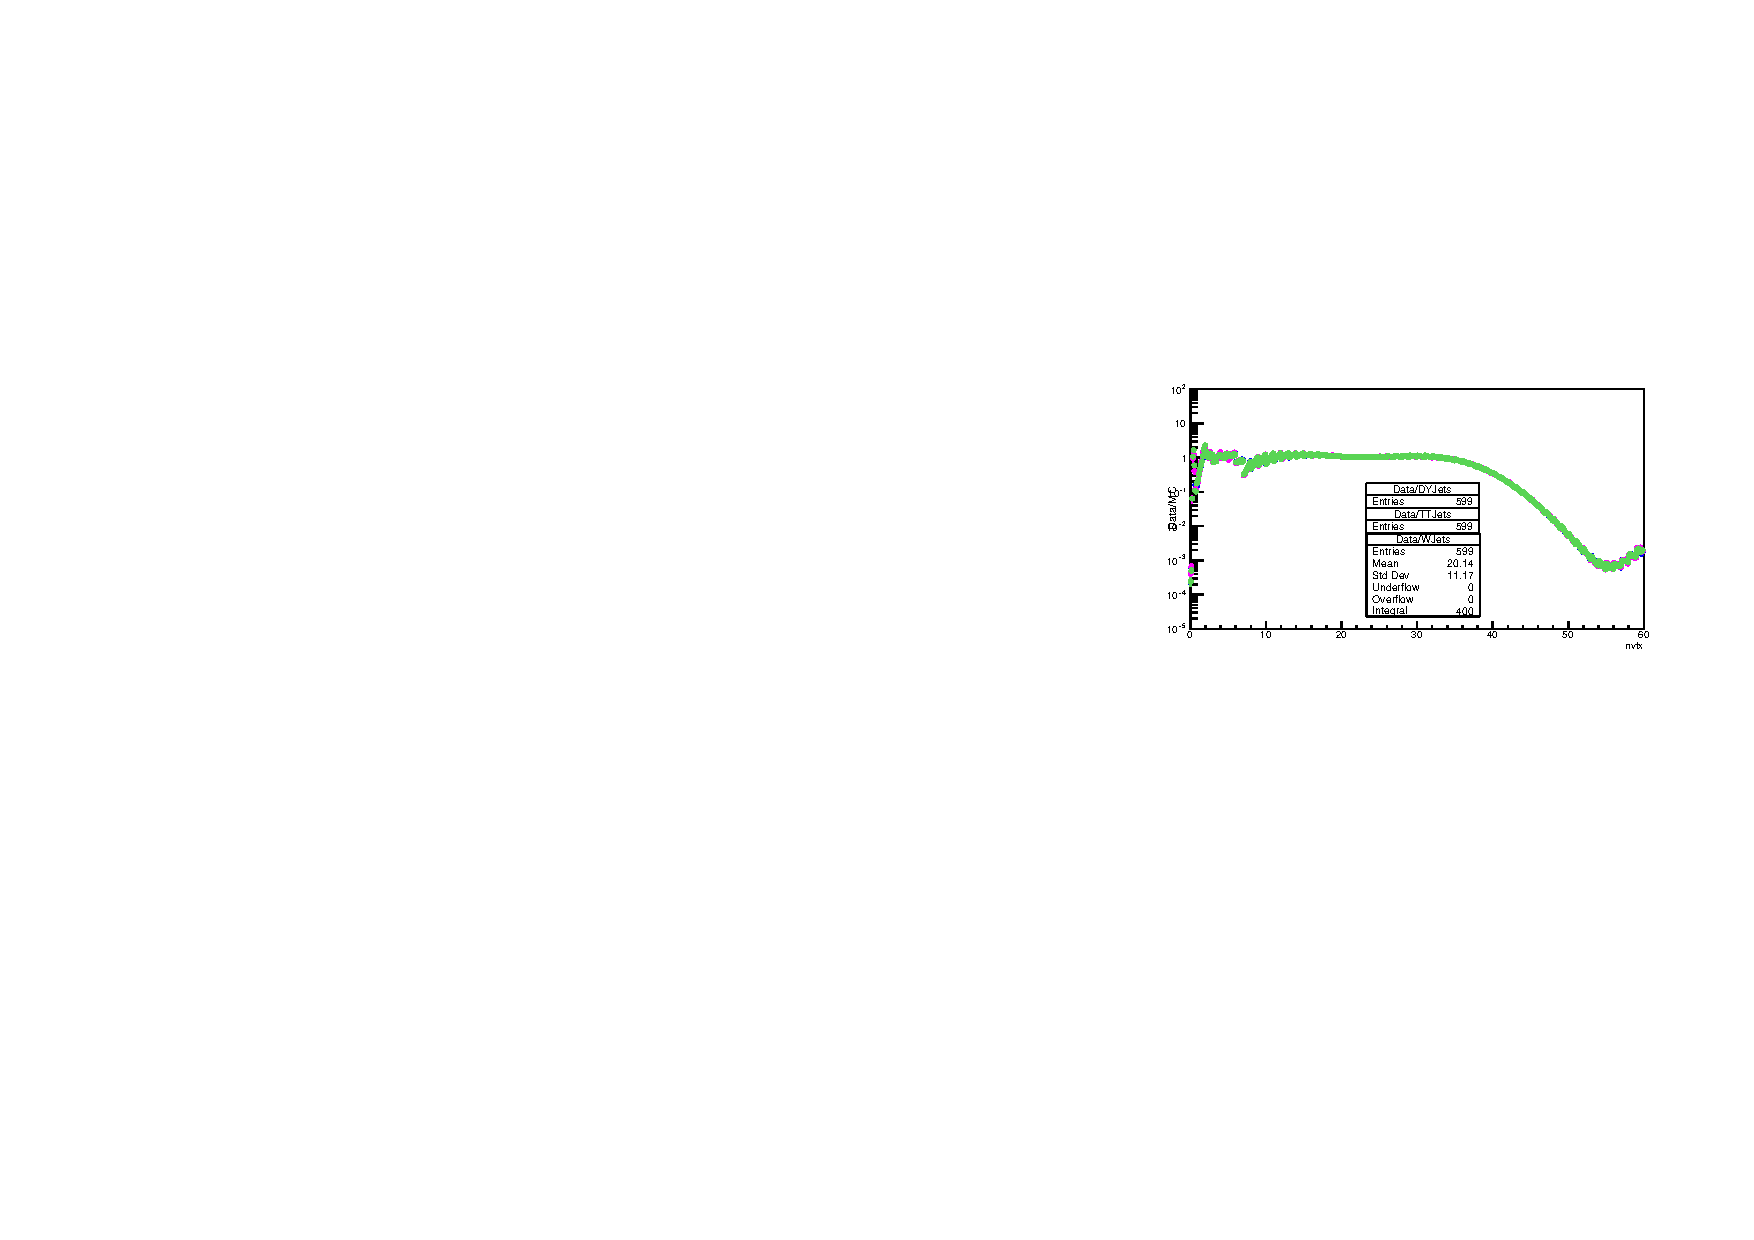
\includegraphics[width=0.60\linewidth]{Image/PU/ratioPileup_all.pdf}}
\caption{ True in-time pileup distribution in (a) \ttjets, (b) $W + jets$,
        (c) $Z/\gamma + jets$ MC samples, and (d) single muon data. The pileup distribution
        is campaign dependent that is why all the MC samples have same pileup distribution as 
    these MC samples were generated in the same campaign.}
\label{fig:mcPileup} 
\end{figure}

\subsection{Lepton Scale Factors}
\label{s:lepton_sf}
Trigger, tracking, isolation and identification efficiencies are different between MC and data.
$\pt$ and $\eta$ dependent scale factors are applied to MC events to take care of this difference.
The 2D histograms used to calculate muon scale factors are shown in Figure~\ref{fig:muSF}.
The muon scale factors are era dependent. There are different muon scale factors for era 
BCDEF and GH. However, electron scale factors are the same for full 2016 data taking period.
The maximum $\pt$ range of 2d-histogram for muon identification and isolation scale factors
is 120 GeV. If a muon has $\pt > 120$ GeV, then the scale factor for $\pt = 120$ GeV is
used. Similarly scale factor of $\pt = 500$ GeV is used for $\pt > 500$
GeV for muon trigger scale factors, and electron scale factors. Separate scale 
factors are combined into one as
\begin{equation}
 SF^\mu = SF^\mu_{\rm ID}\times SF^\mu_{\rm iso}\times SF^\mu_{\rm track}\times SF^\mu_{\rm trig}, \quad
 SF^{ele} = SF^{ele}_{\rm ID}\times SF^{ele}_{\rm reco}\times SF^{ele}_{\rm trig},
\label{eq:lepSF}
\end{equation}
where $SF^\mu_{\rm ID}$, $SF^\mu_{\rm iso}$, $SF^\mu_{\rm track}$ and $SF^\mu_{\rm trig}$ are weighted
average with luminosity ($L$) for different eras (Run-BCDEF and Run-GH) e.g. 
\begin{equation}
 SF^\mu_{\rm ID}=\frac{SF^\mu_{\rm ID}({\rm BCDEF})\times L({\rm BCDEF})+SF^\mu_{\rm ID}({\rm GH})\times L({\rm GH})}
 {L({\rm BCDEF})+L({\rm GH})}.
\end{equation}
Where, for example, $SF^\mu_{\rm ID}({\rm BCDEF})$ is the scale factor for 
Run-B to Run-F and L({\rm BCDEF})
is the luminosity during this period. A similar formula for $SF^\mu_{\rm iso}$, 
$SF^\mu_{\rm track}$ and $SF^\mu_{\rm trig}$ is used. The scale factors of 
Eq.~(\ref{eq:lepSF}) are applied on MC events.
\begin{center}
\begin{figure}
    \subfigure[ID scale factors for run BCDEF]
    {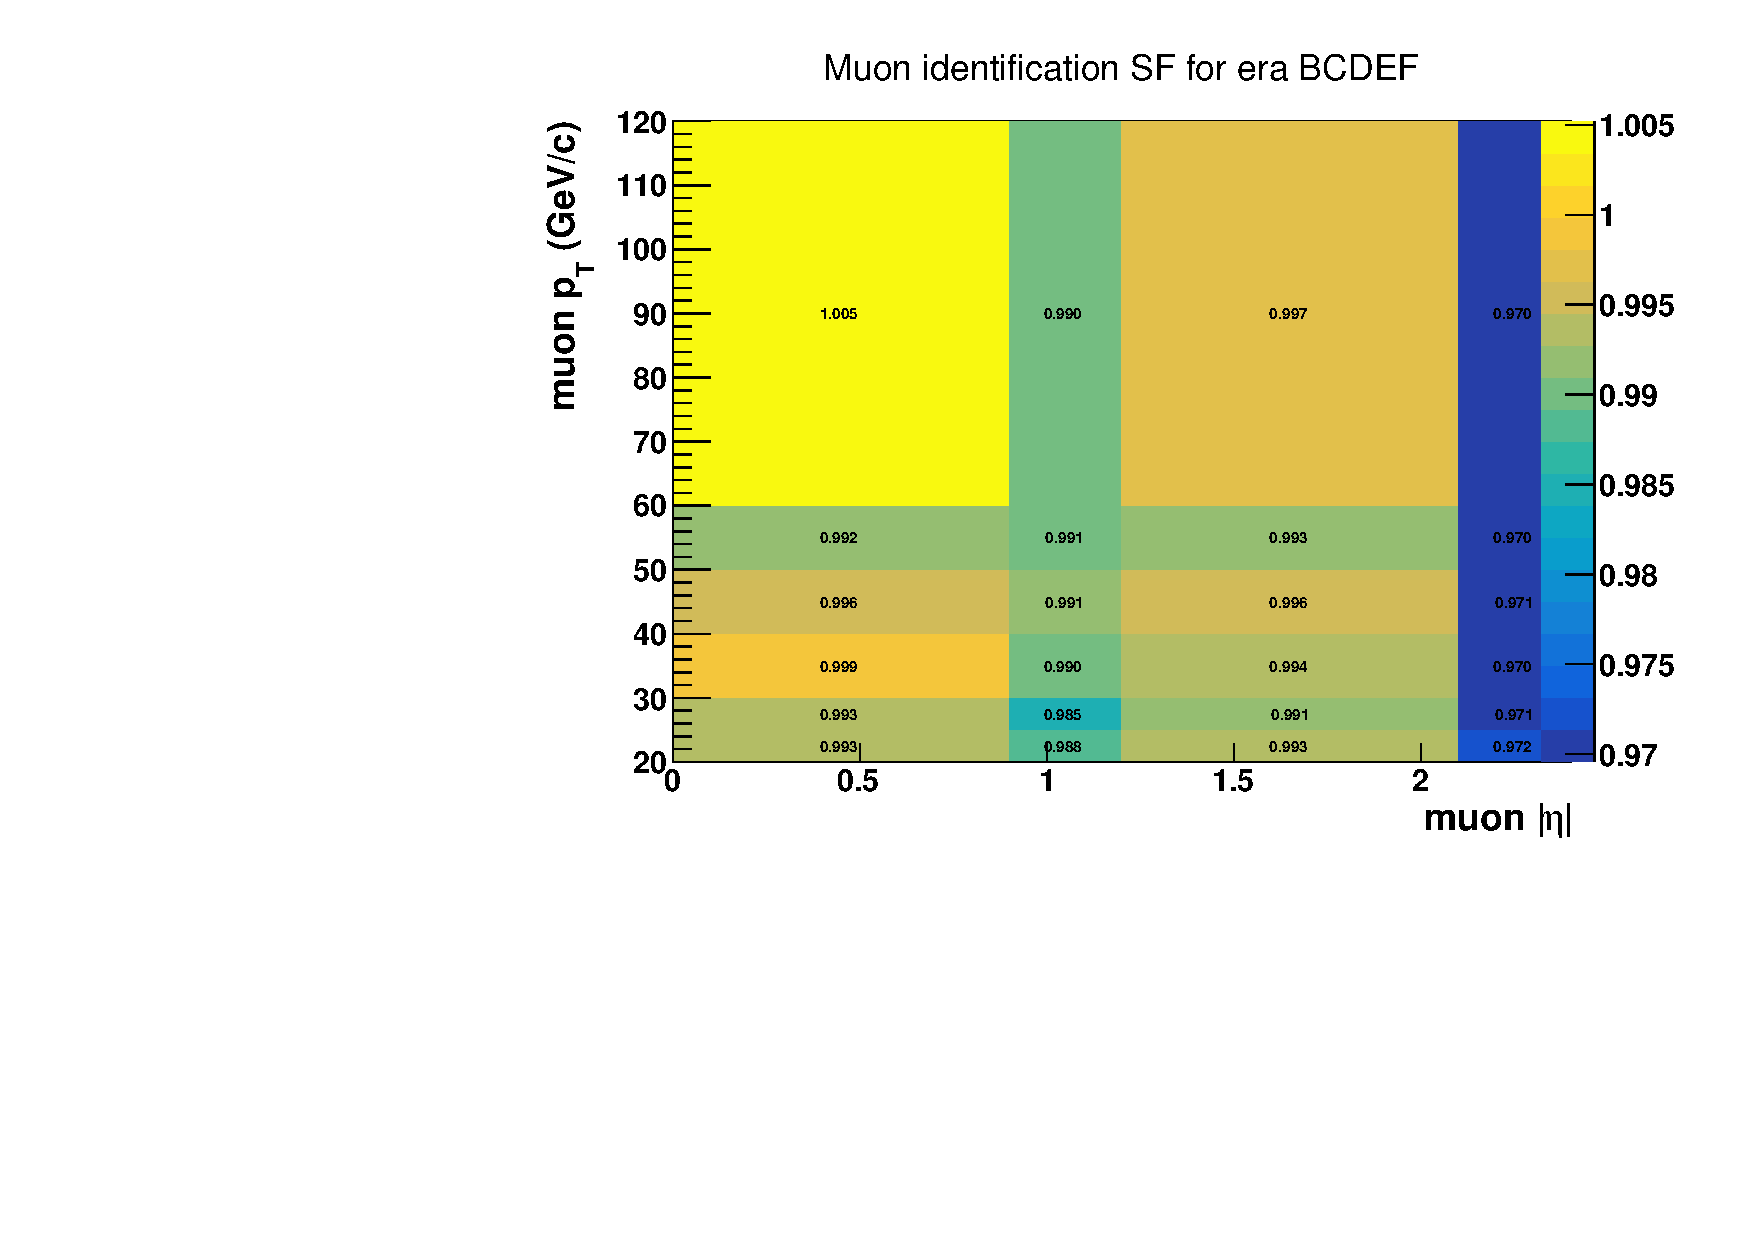
\includegraphics[width=0.45\linewidth]{Image/EffAndSF/mu_idSF_BCDEF.pdf}}
    \subfigure[ID scale factors for run GH]
    {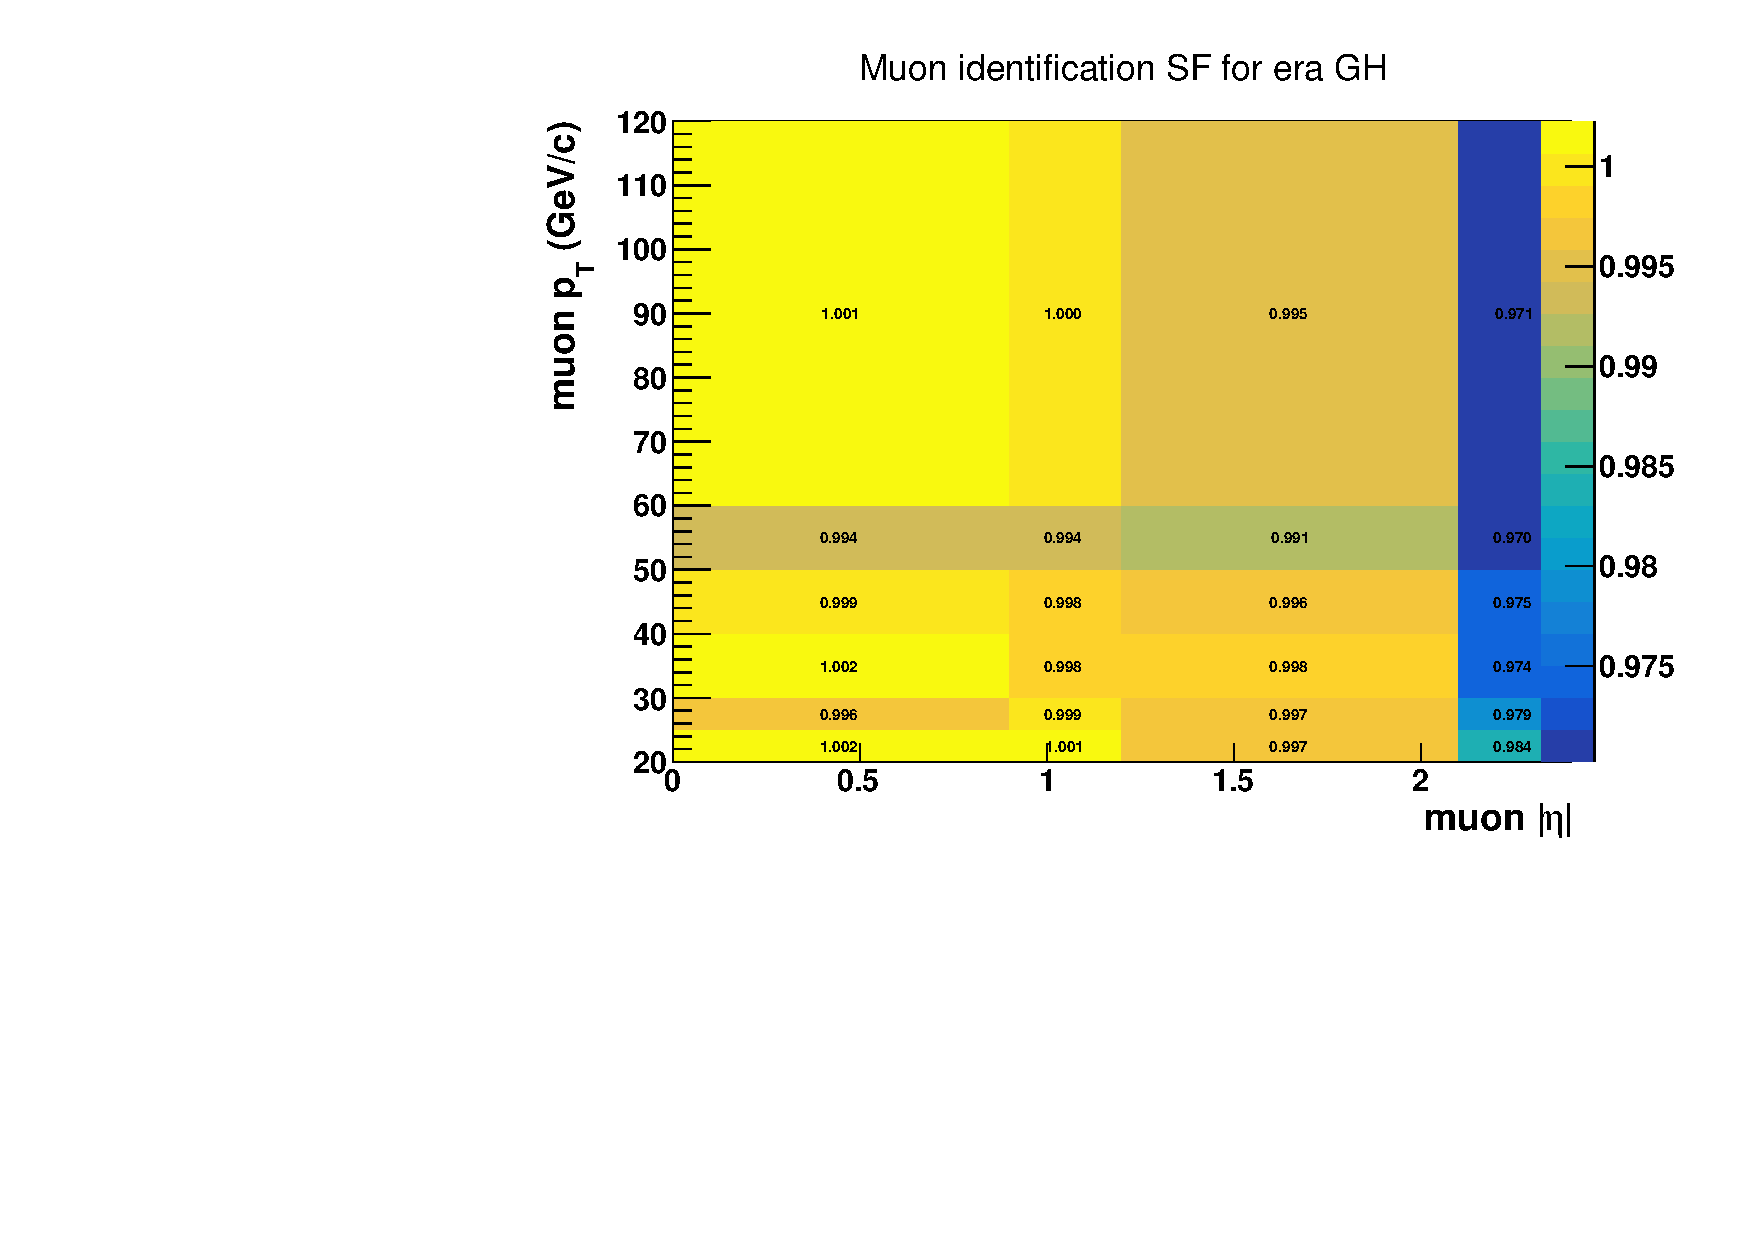
\includegraphics[width=0.45\linewidth]{Image/EffAndSF/mu_idSF_GH.pdf}}
    \vfil
    \subfigure[Iso scale factors for run BCDEF]
    {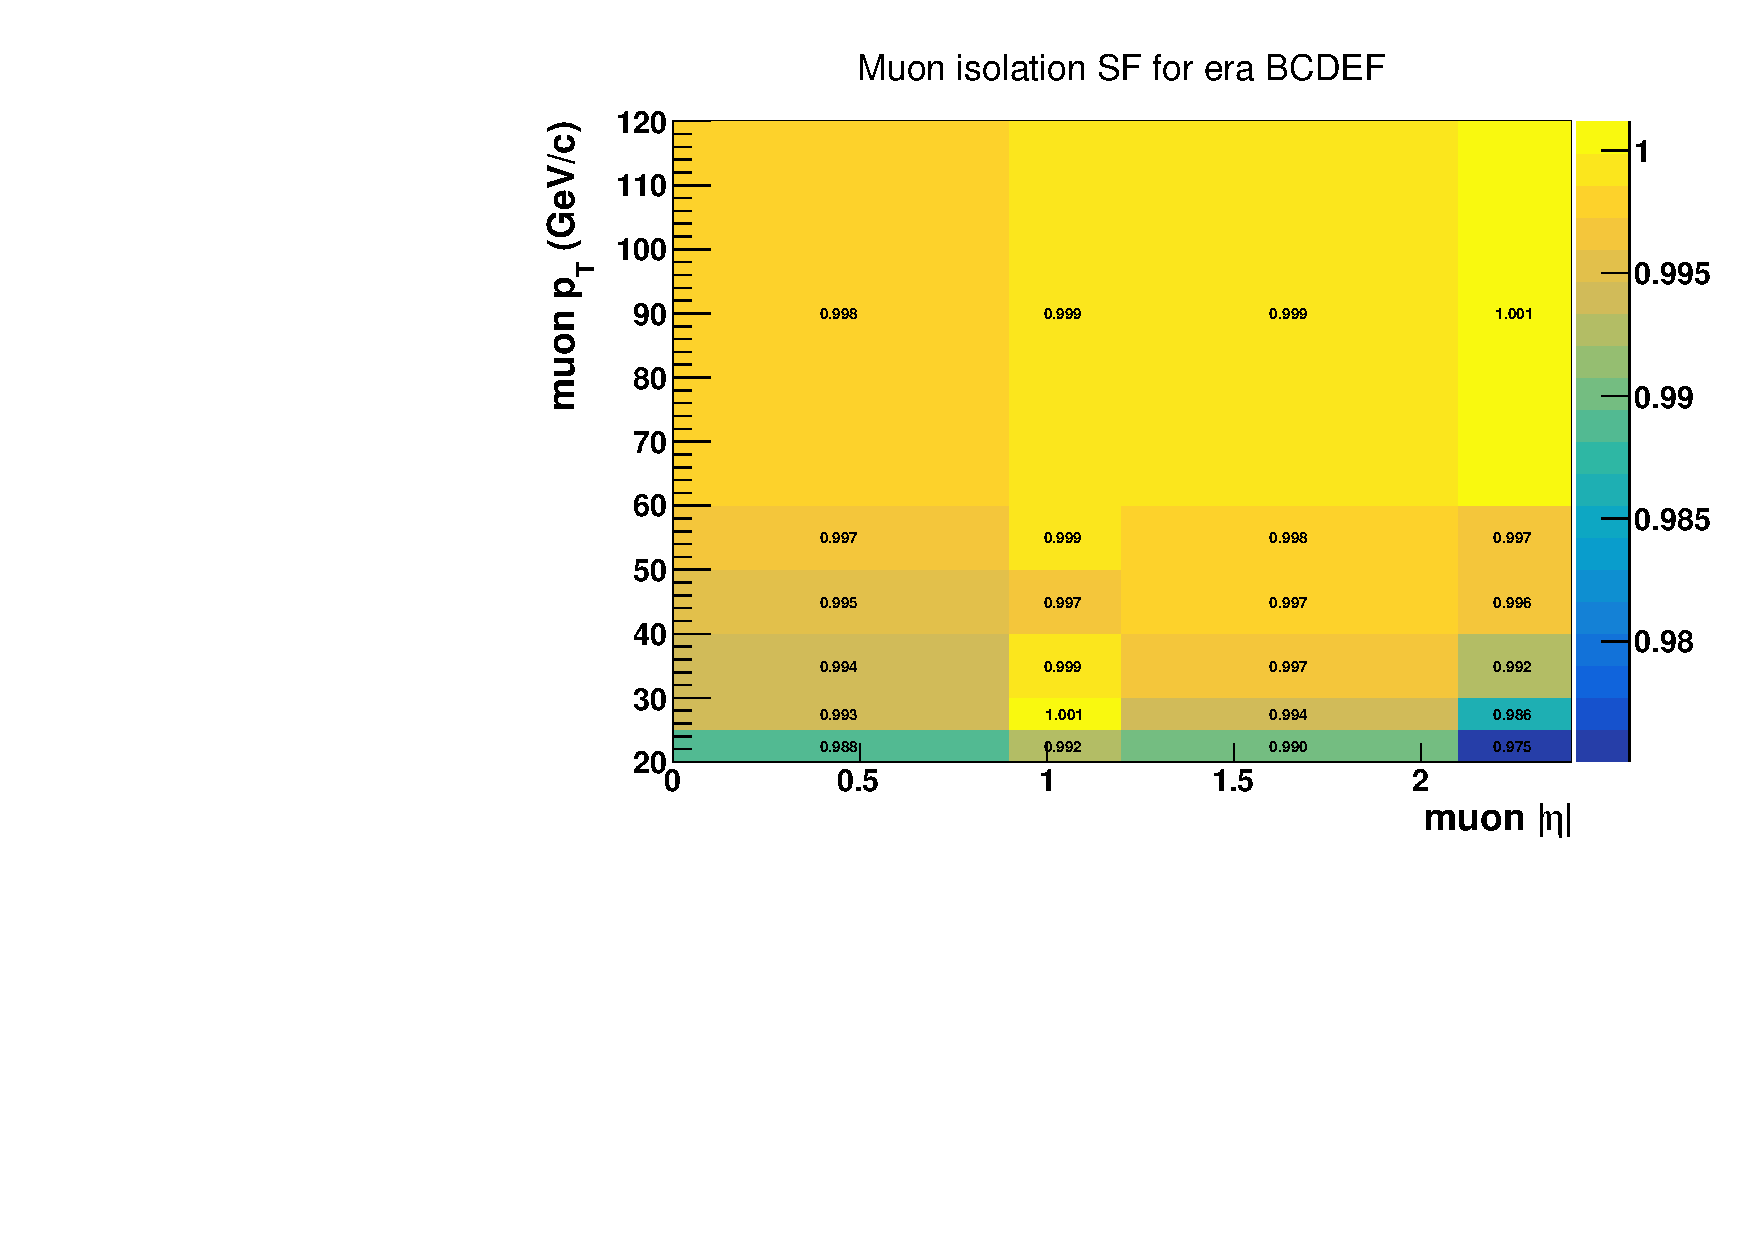
\includegraphics[width=0.45\linewidth]{Image/EffAndSF/mu_isoSF_BCDEF.pdf}}
    \subfigure[Iso scale factors for run GH]
    {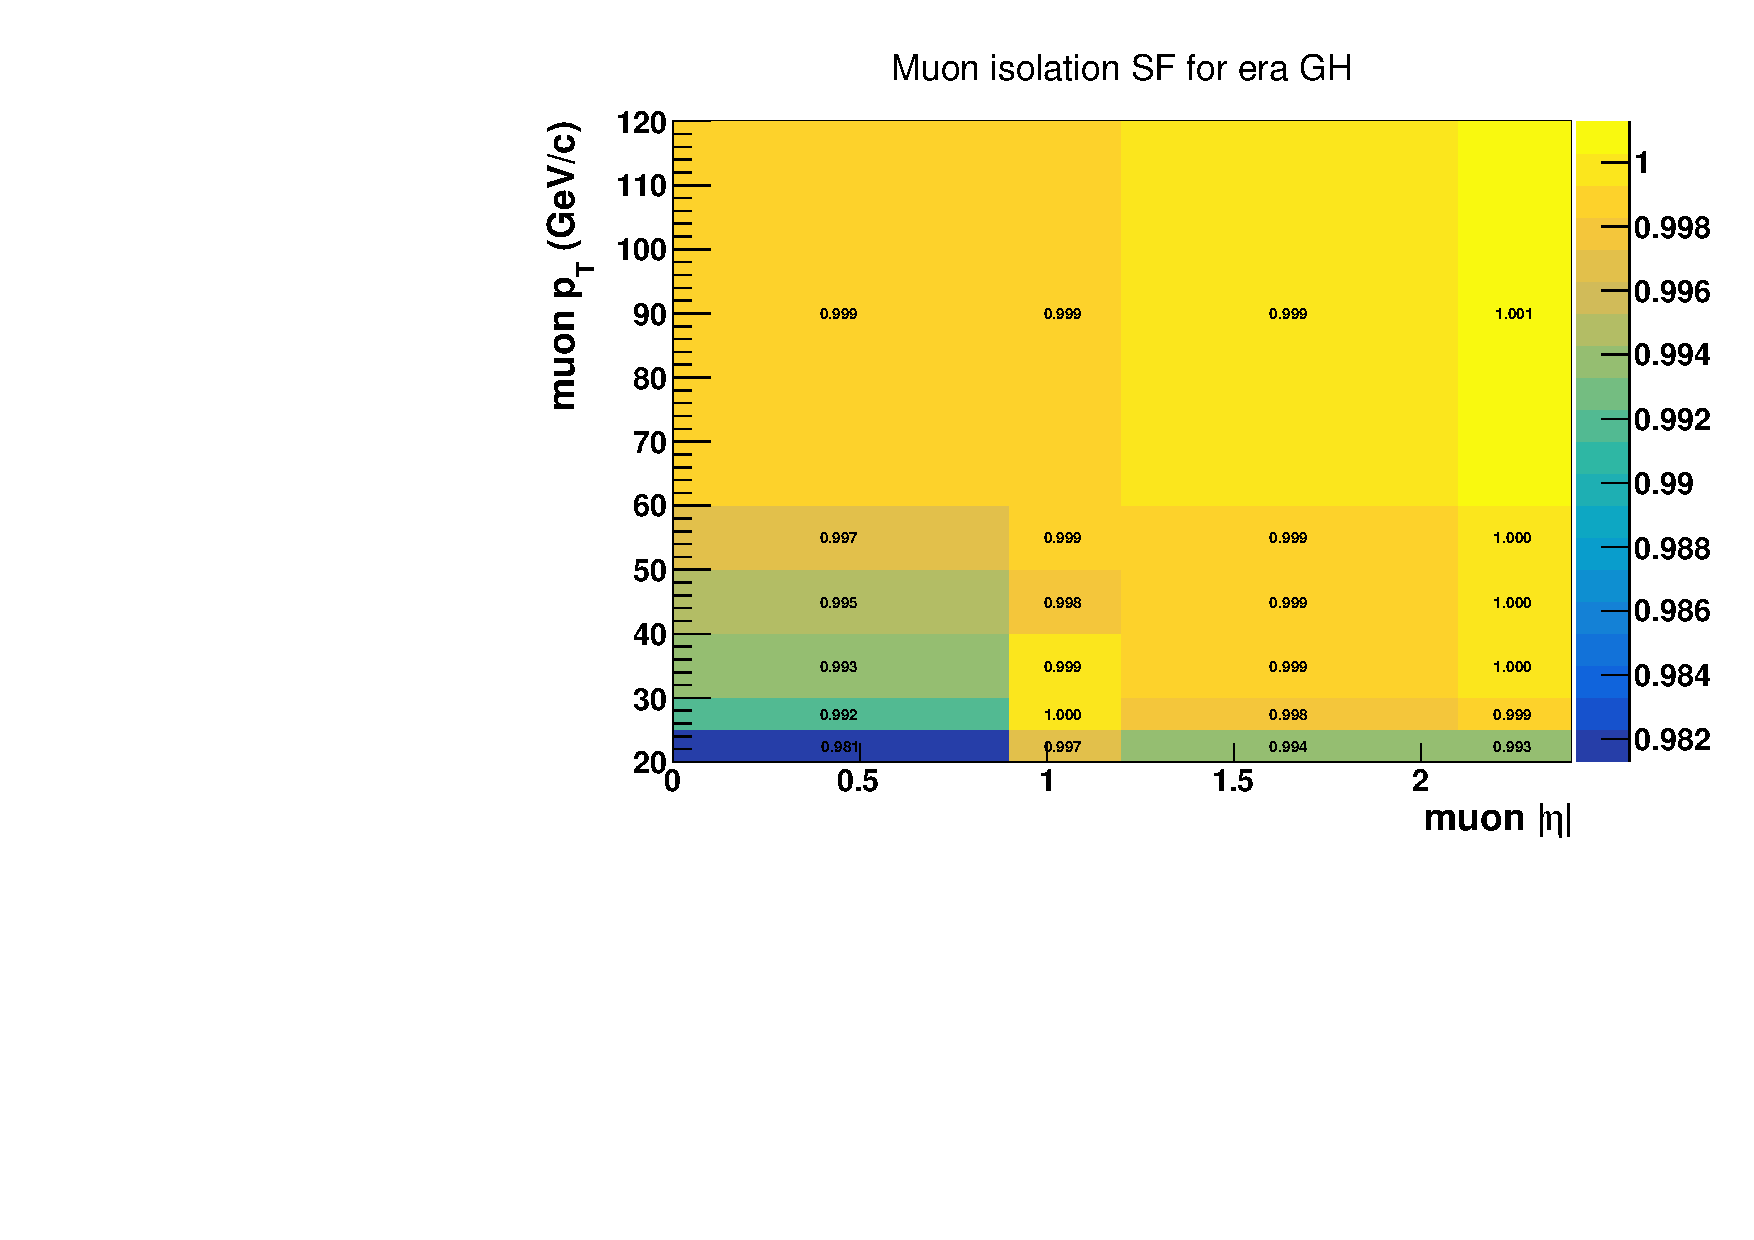
\includegraphics[width=0.45\linewidth]{Image/EffAndSF/mu_isoSF_GH.pdf}}
    \vfil
    \subfigure[Tracking scale factors for run BCDEF]
    {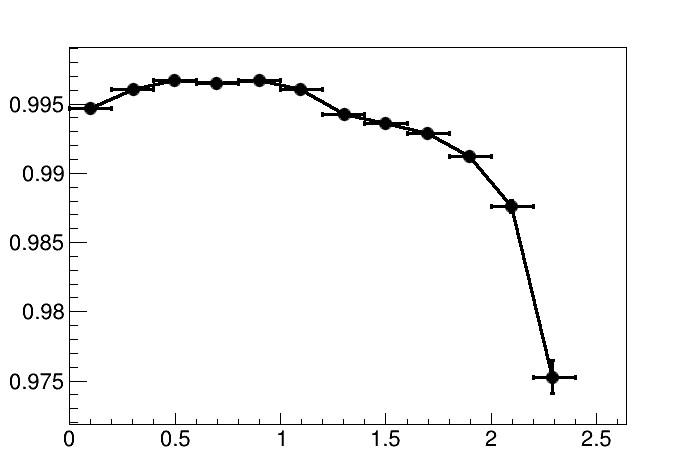
\includegraphics[width=0.45\linewidth]{Image/EffAndSF/mu_trackSF_BCDEF.png}}
    \subfigure[Tracking scale factors for run GH]
    {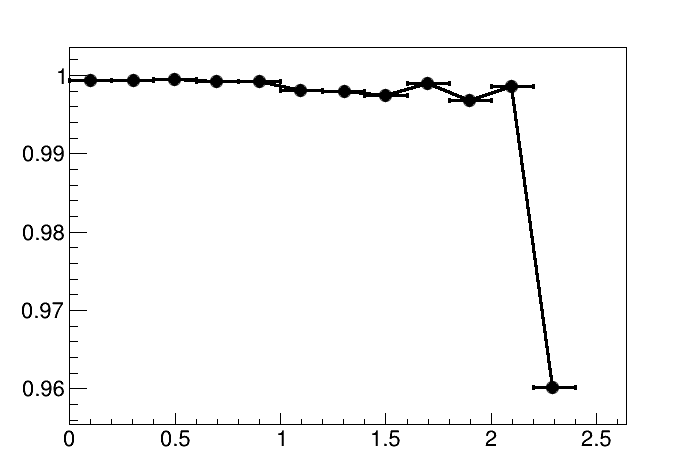
\includegraphics[width=0.45\linewidth]{Image/EffAndSF/mu_trackSF_GH.png}}
    \vfil
    \subfigure[Trigger scale factors for run BCDEF]
    {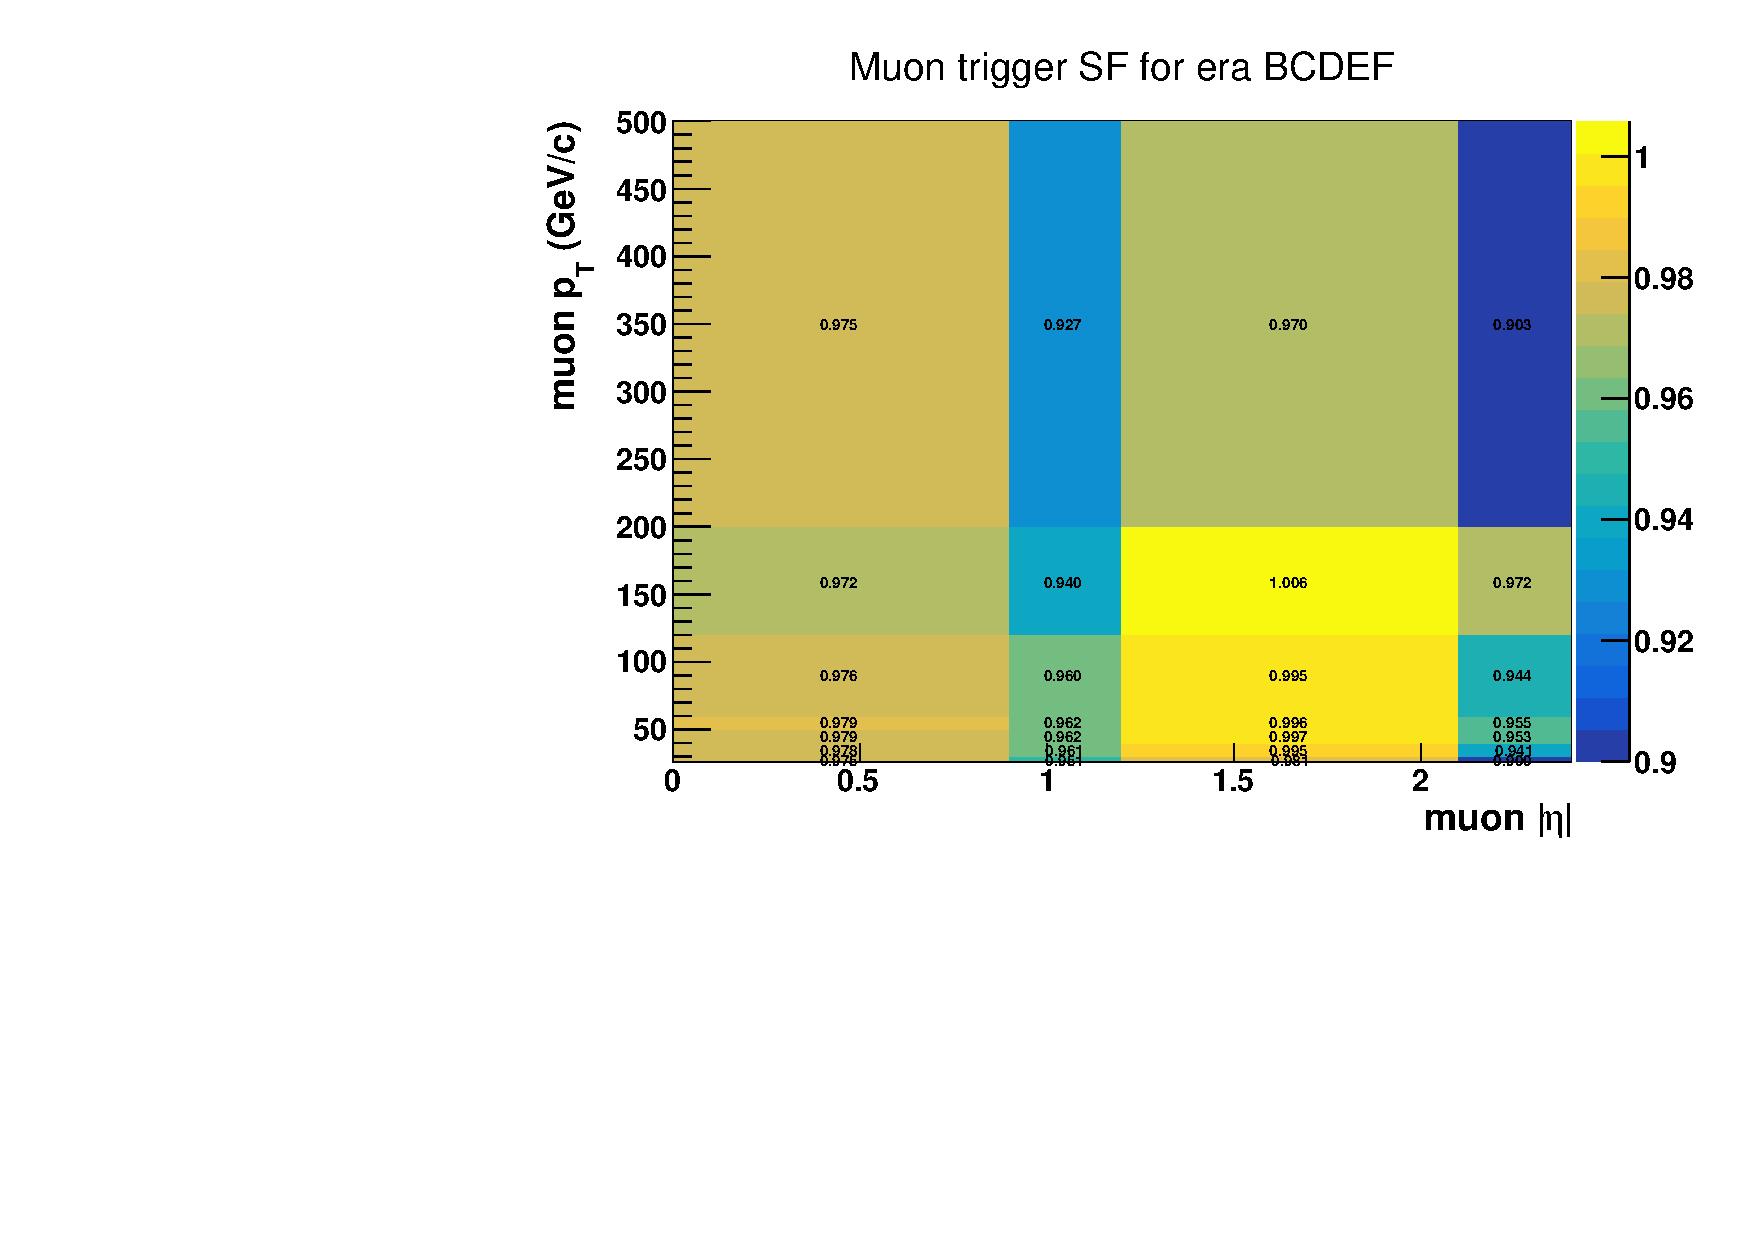
\includegraphics[width=0.45\linewidth]{Image/EffAndSF/mu_trigSF_BCDEF.pdf}}
    \subfigure[Trigger scale factors for run GH]
    {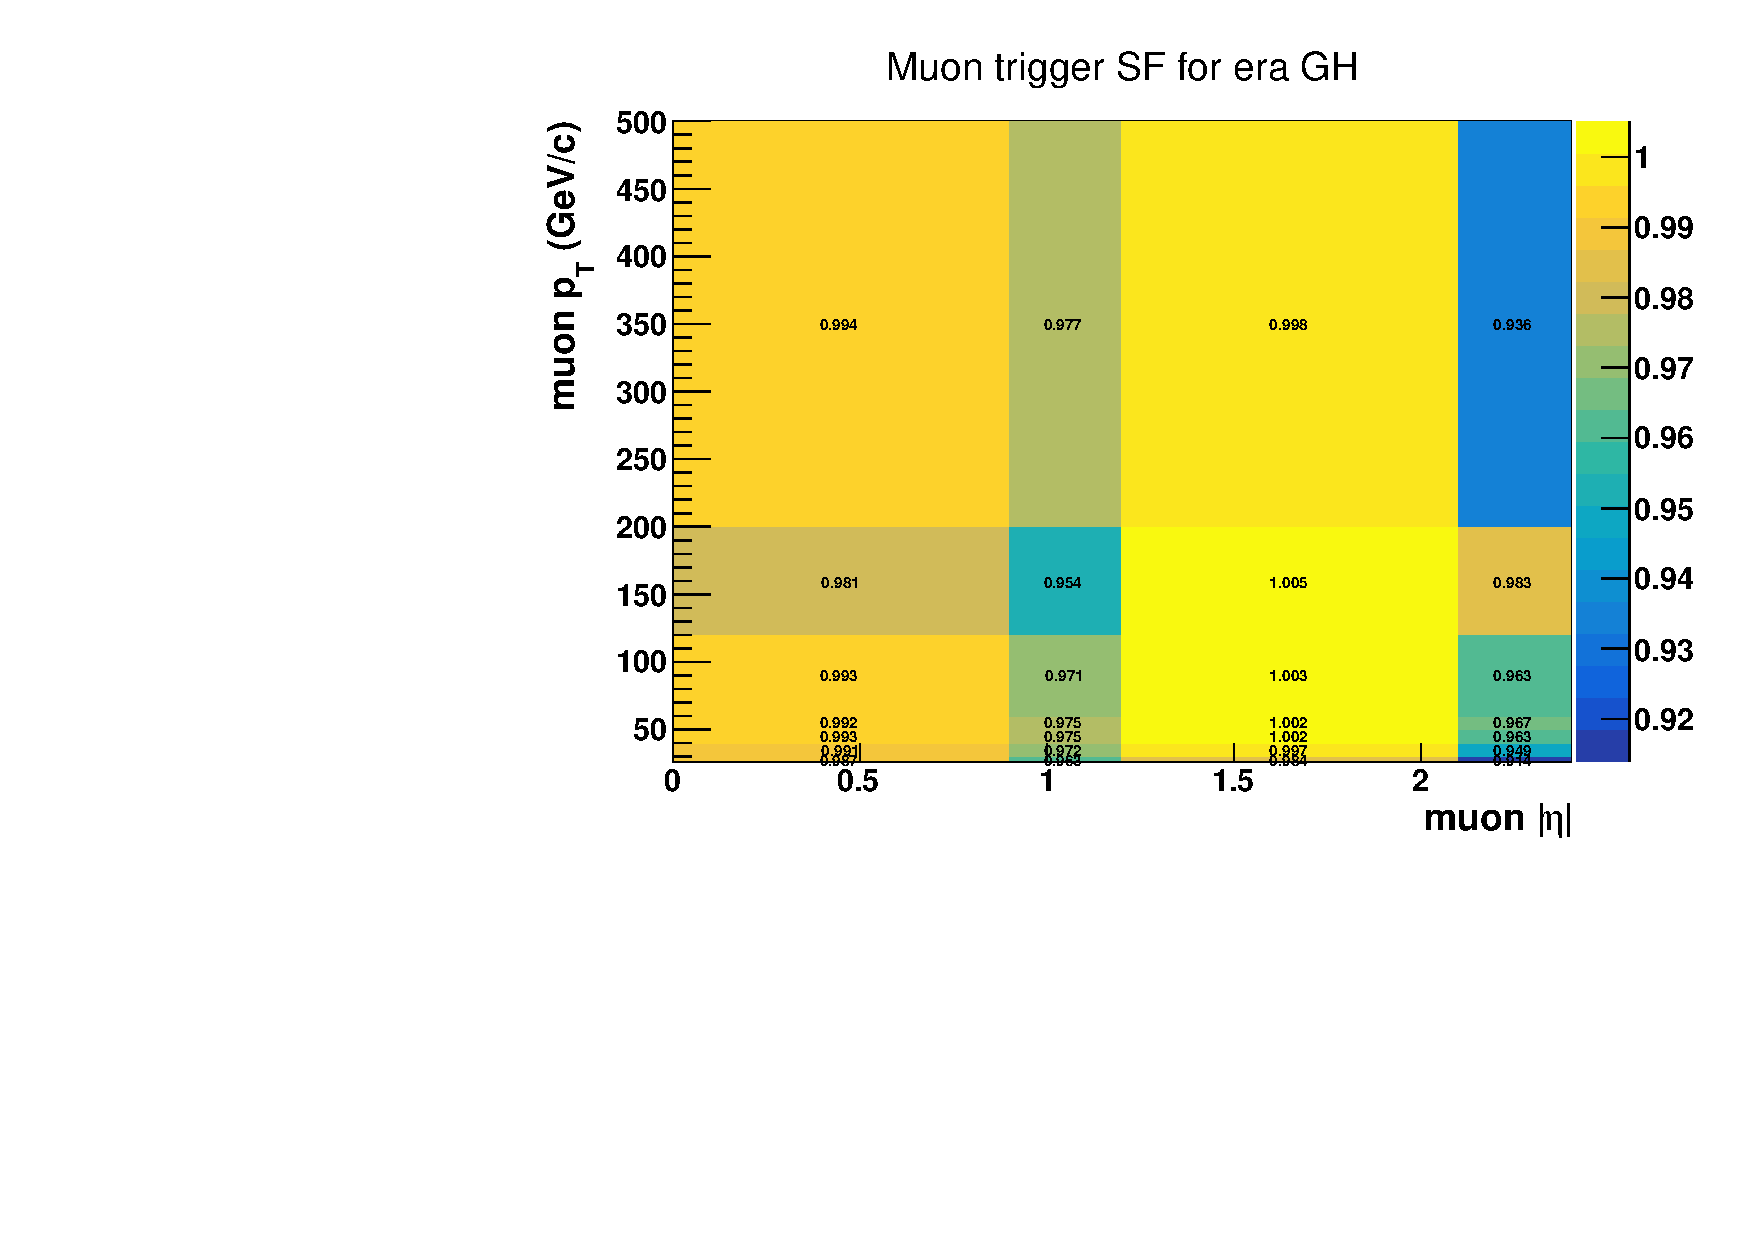
\includegraphics[width=0.45\linewidth]{Image/EffAndSF/mu_trigSF_GH.pdf}}
\caption{ Identification, isolation, tracking and trigger scale factors for muon.} 
\label{fig:muSF}
\end{figure}
\end{center}
The electron scale factors, as shown in Figure~\ref{fig:eleSF} are read from 
2D histograms provide by~\cite{eleSF}.
\begin{center}
\begin{figure}
   \subfigure[ Medium ID scale factors]
   {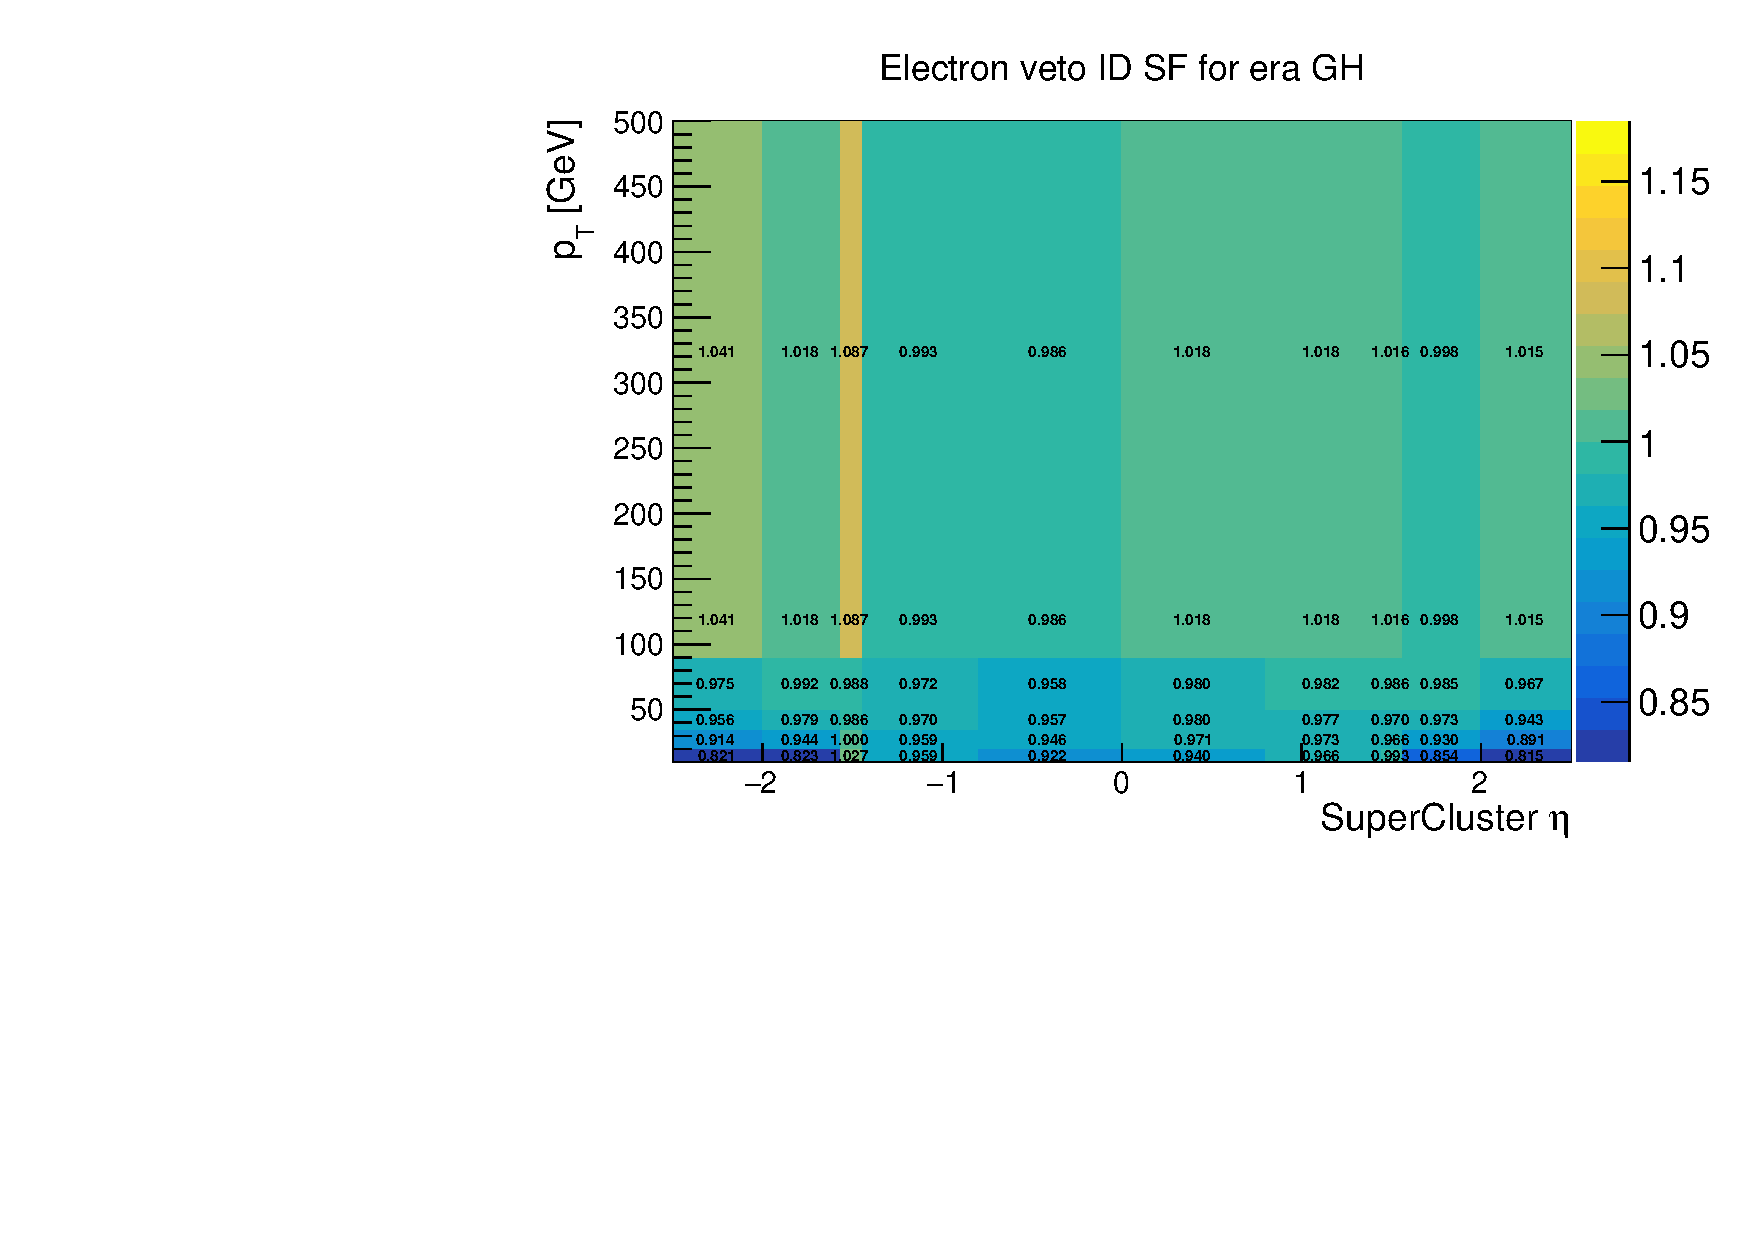
\includegraphics[width=0.45\linewidth]{Image/EffAndSF/ele_medium_idSF.pdf}}
   \subfigure[ Veto ID scale factors ]
   {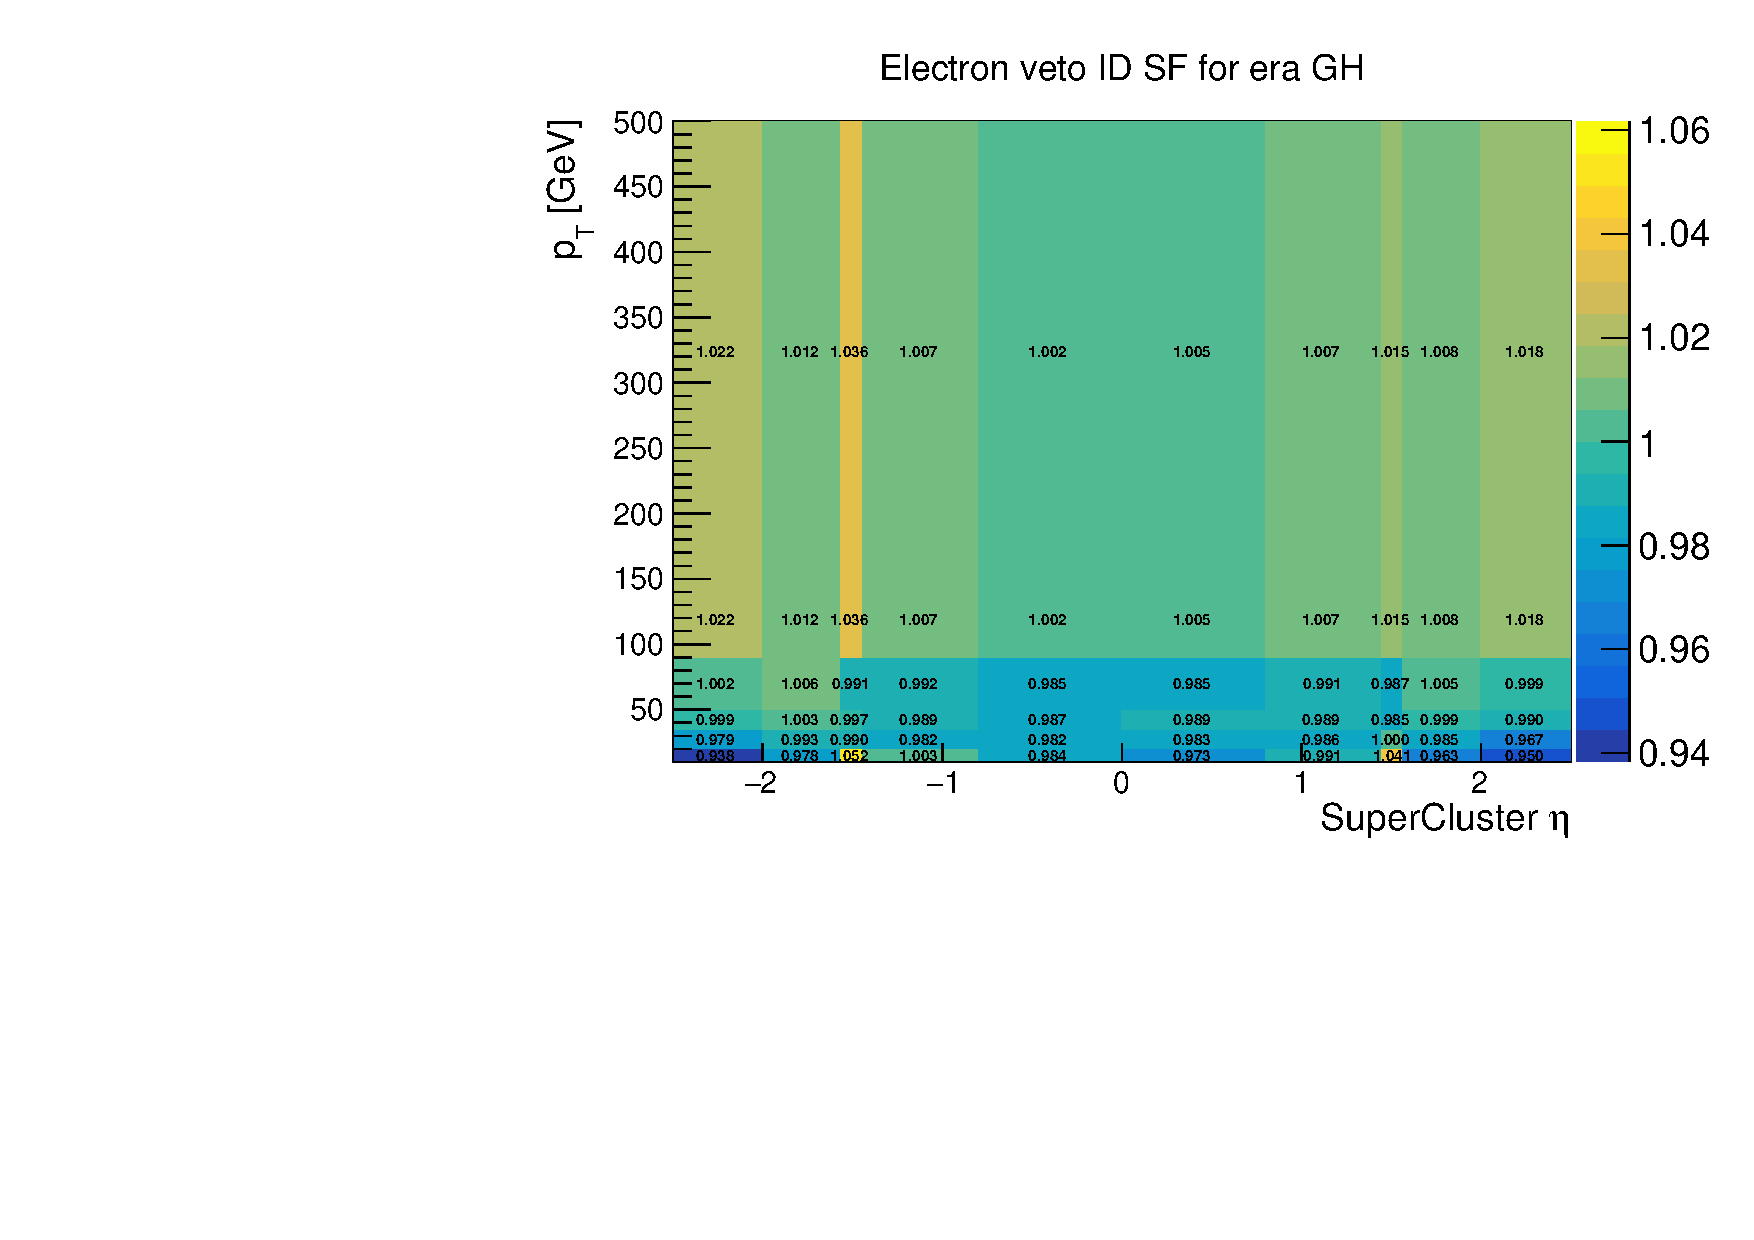
\includegraphics[width=0.45\linewidth]{Image/EffAndSF/ele_veto_idSF.pdf}}
   \vfil
   \subfigure[ Reconstruction scale factors]
   {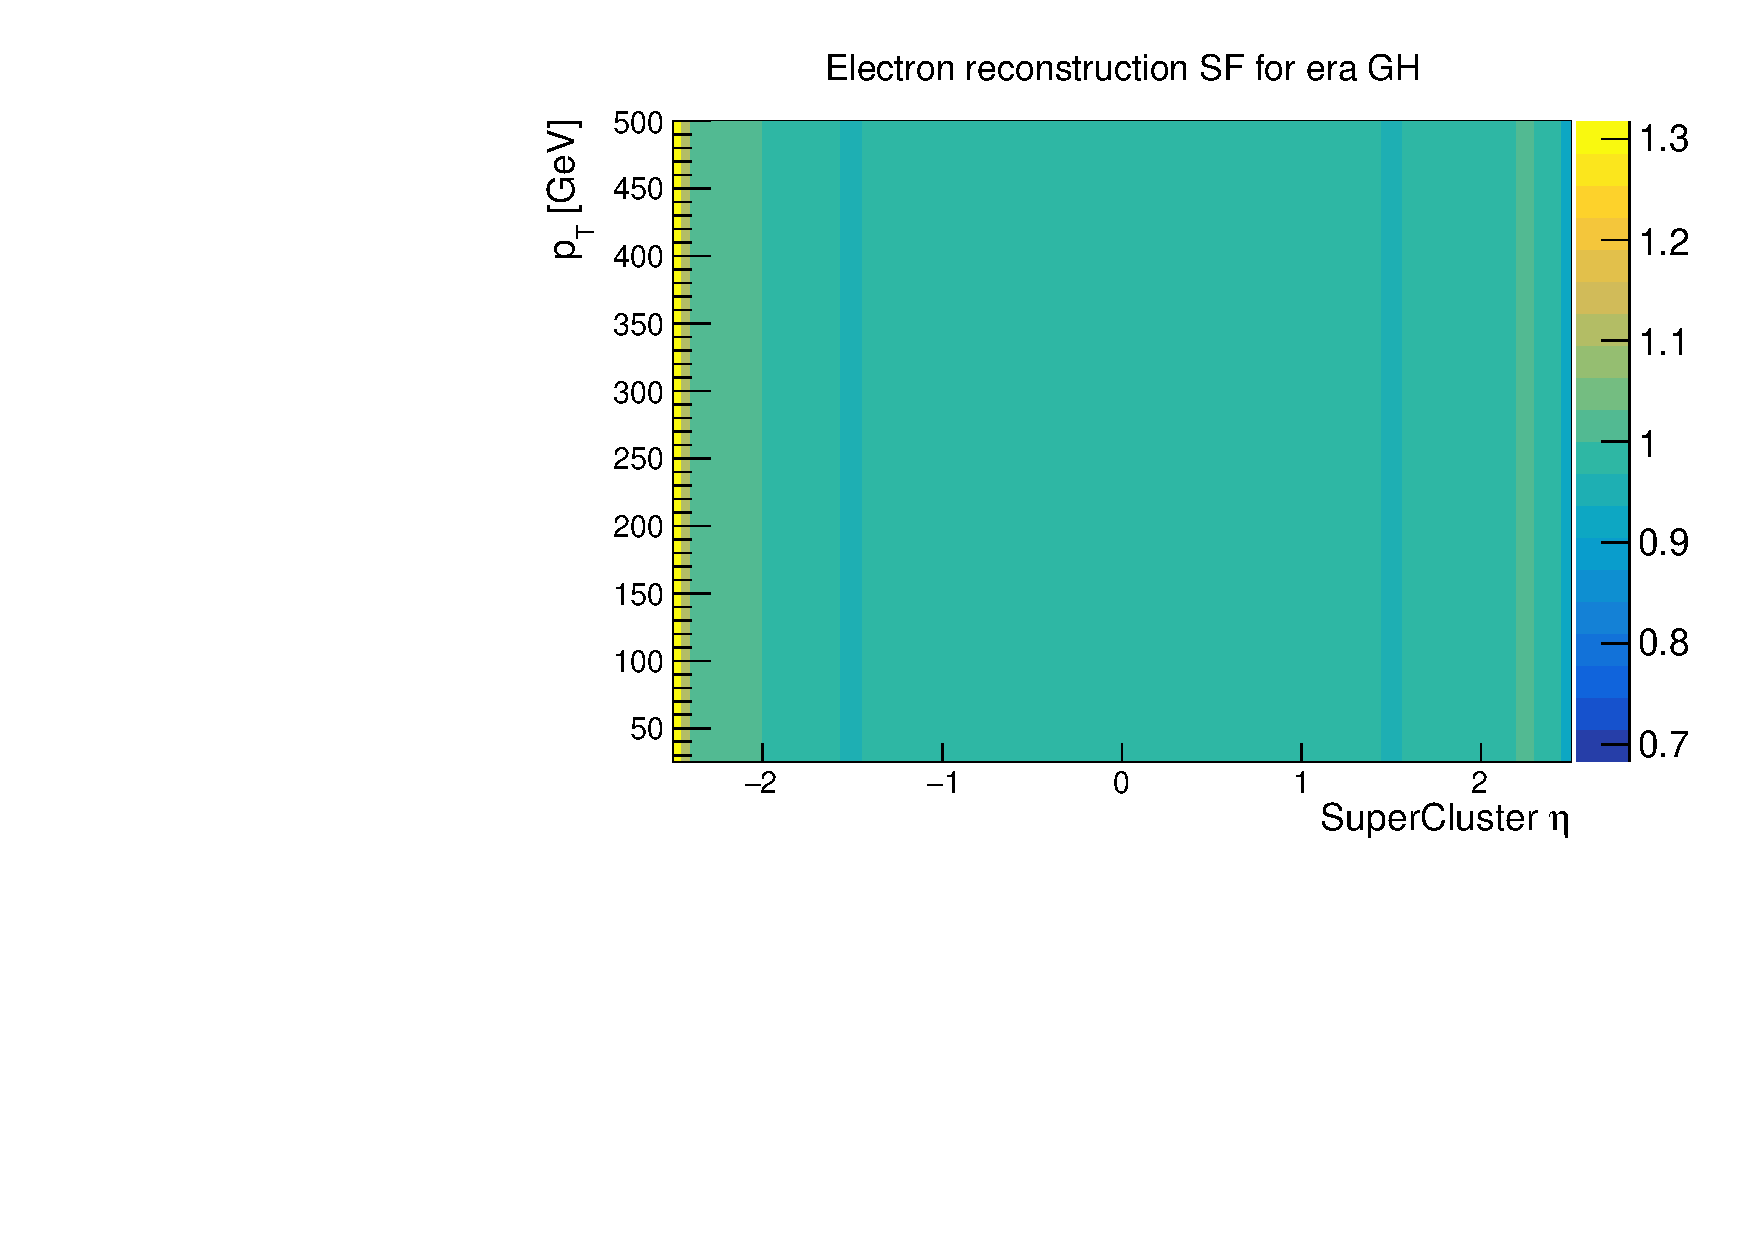
\includegraphics[width=0.45\linewidth]{Image/EffAndSF/ele_recoSF.pdf}}
   \subfigure[ Trigger scale factors]
   {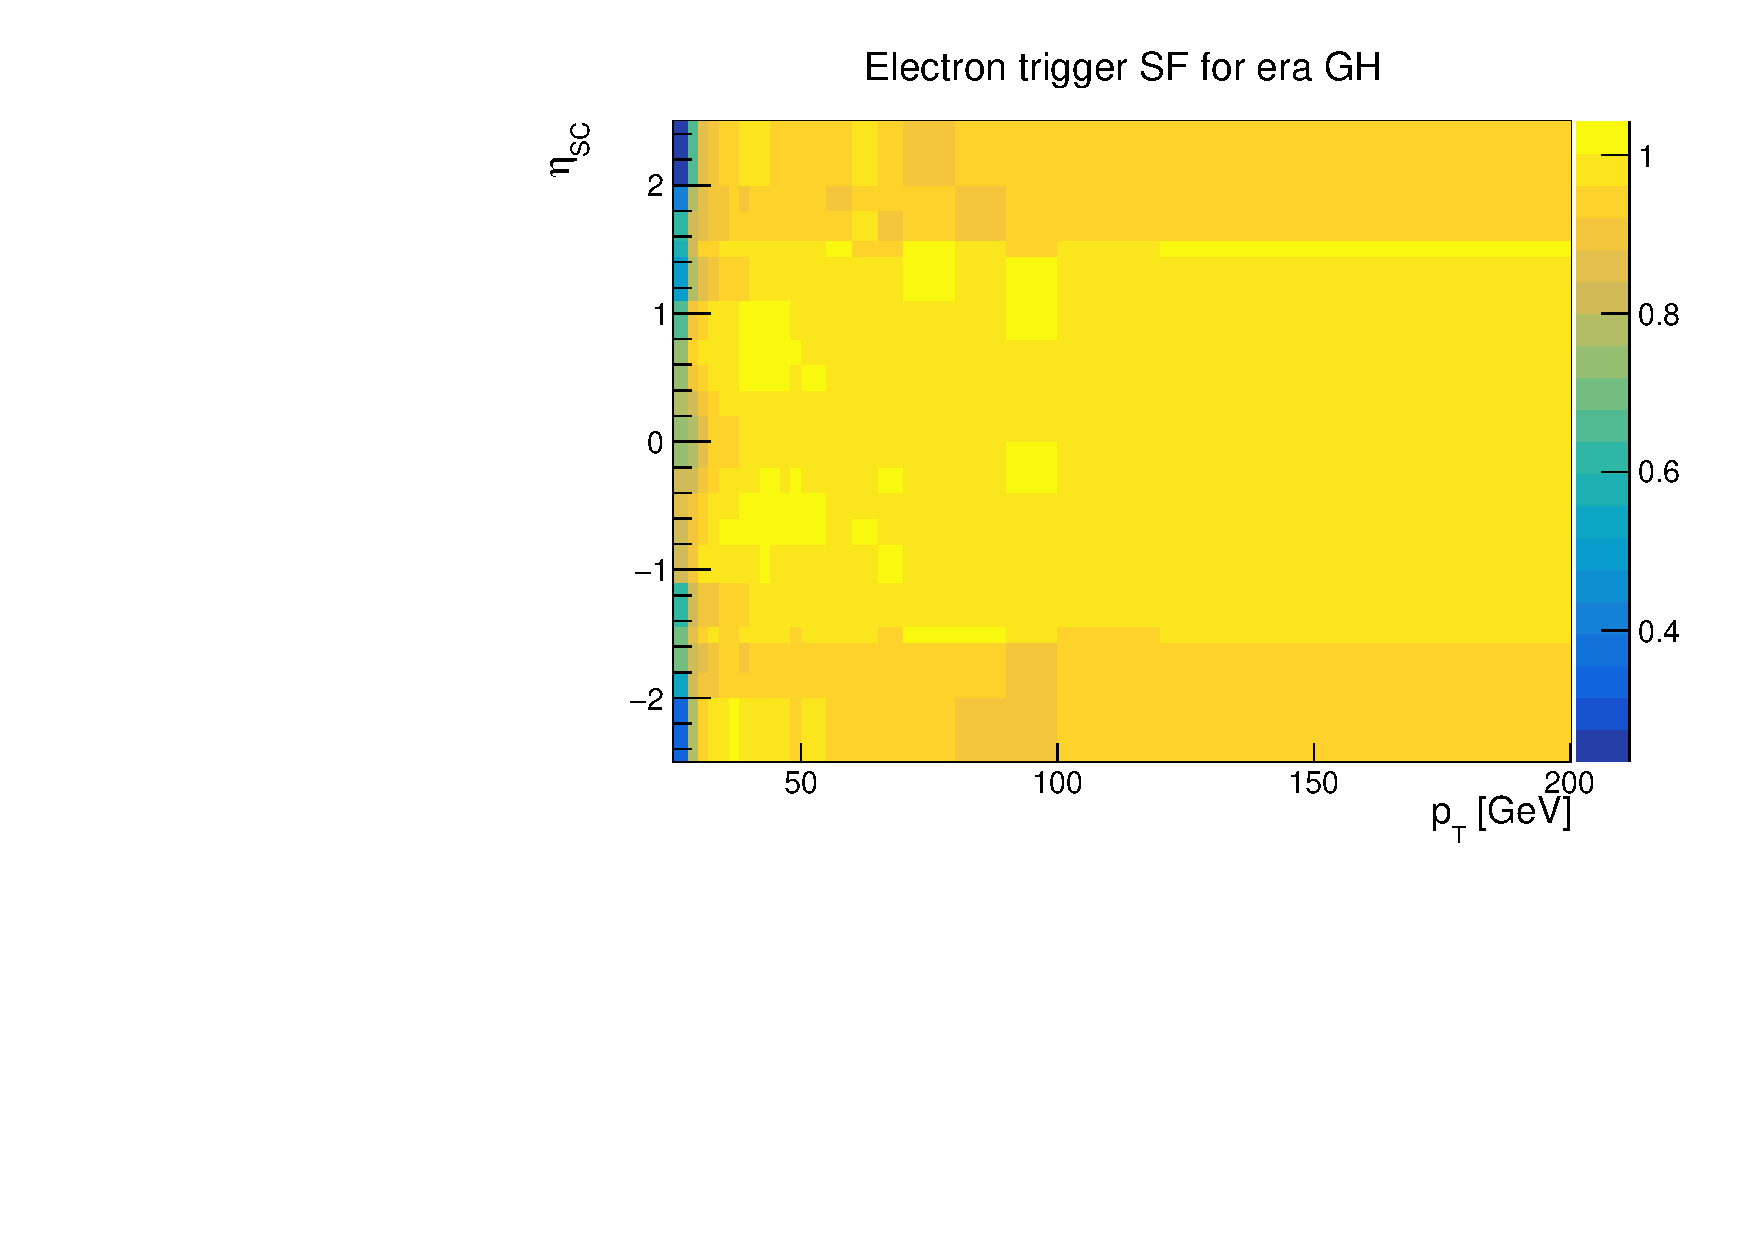
\includegraphics[width=0.45\linewidth]{Image/EffAndSF/ele_trigSF.pdf}}
\caption{ Identification, Reconstruction and Trigger scale factors for electron.} 
\label{fig:eleSF}
\end{figure}
\end{center}

\subsection{Jet and MET Correction}
\label{s:JEC}
Jets from simulations are smeared using jet energy scale (JES) and jet energy 
resolution (JER) to have the same resolution as that in data~\cite{Khachatryan:2016kdb}.
For smearing $\pt$ and $\eta$ dependent scale factors ($SF$) are used as listed 
in Table~\ref{tab:jer_sf}. The $\pt$ of jet in simulations is scaled by the 
following factor:
\begin{equation}
    {\pt}_{scale} = {\rm
    max}[0.0,1.0+(SF-1)\times({\pt}_{jet}-{\pt}_{jet}^{gen})/{\pt}_{jet}]
\end{equation}
with the following constraint:
\begin{equation}
    {\pt}_{jet}^{gen}> 0, \quad \Delta R<0.2, \quad |{\pt}_{jet}-{\pt}_{jet}^{gen} |<
    3\times\sigma_{\rm JER}\times{\pt}_{jet},
\end{equation}
where $\Delta R$ is the angular separation between the reconstructed and 
generated jet and $\sigma_{JER}$ is resolution of reconstructed jet-\pt, calculated using
\verb|Spring16_25nsV10_MC_PtResolution_AK4PF.txt| and global tag \verb|80X_mcRun2_asymptotic| \verb|_2016_TrancheIV_v10|. 
\begin{table}
    \caption{Jet energy resolution scale factors for different $\eta$ range}
 \label{tab:jer_sf}
 \begin{center}
 \begin{tabular}{cccc}
     \hline
     \hline
     $\eta$ range & base & down & up \\ 
     \hline
     \hline
     $0.0 \leq | \eta |< 0.5 $ & 1.109 & 1.044 & 1.174 \\
     $0.5 \leq | \eta |< 0.8 $ & 1.138 & 1.072 & 1.204 \\
     $0.8 \leq | \eta |< 1.1 $ & 1.114 & 1.050 & 1.178 \\
     $1.1 \leq | \eta |< 1.3 $ & 1.123 & 1.022 & 1.224 \\
     $1.3 \leq | \eta |< 1.7 $ & 1.084 & 0.985 & 1.183 \\
     $1.7 \leq | \eta |< 1.9 $ & 1.082 & 0.973 & 1.191 \\
     $1.9 \leq | \eta |< 2.1 $ & 1.140 & 1.020 & 1.260 \\
     $2.1 \leq | \eta |< 2.3 $ & 1.067 & 0.953 & 1.181 \\
     $2.3 \leq | \eta |< 2.5 $ & 1.177 & 0.967 & 1.387 \\
     $2.5 \leq | \eta |< 2.8 $ & 1.364 & 1.203 & 1.525 \\
     $2.8 \leq | \eta |< 3.0 $ & 1.857 & 1.654 & 2.060 \\
     $3.0 \leq | \eta |< 3.2 $ & 1.328 & 1.203 & 1.453 \\
     $3.2 \leq | \eta |< 5.0 $ & 1.160 & 1.013 & 1.307 \\ \hline
 \end{tabular}
 \end{center}
 \end{table}

\subsection{b-tag Scale Factor}
\label{s:bTagSF}
The b-tagging efficiency is different between MC and data.
An event weight as given by Eq.\ref{eq:btagWt} is applied on the simulated events to 
take care of this difference ~\cite{BTagSFMethods}. 
\begin{equation}
P(MC) = \prod_{i = tagged} \epsilon_i \prod_{j = not \, tagged}(i -\epsilon_j)
\end{equation}
\begin{equation}
P(Data) = \prod_{i=tagged} SF_{i}\epsilon_i \prod_{j = not \, tagged} (1-SF_j\epsilon_j)
\end{equation}
\begin{equation}
w = \frac{P(Data)}{P(MC)}
\label{eq:btagWt}
\end{equation}
 The b-tag efficiency $\epsilon_f(m,n)$ in the $(m,n)$ bin of $\pt$ and $\eta$ is calculated 
 using the following formula                                                               
 \begin{equation}                                                                          
  \epsilon_f(m,n)=\frac{N^{\rm b-tagged}_f(m,n)}{N^{\rm total}_f(m,n)},                   
 \label{eq:btag_eff}                                                                       
 \end{equation}                                                                            
 where $N^{\rm b-tagged}_f(m,n)$ is the number of b-tagged jets with flavor $f$ (b-quark, c-quark,
 light-quark and gluon) and $N^{\rm total}_f(m,n)$ is the total number of events. The scale factor ($SF_i$) 
 depends on $\pt$, $\eta$, parton-flavor of jet and b-jet discriminator value,
 and are read from \verb|CSVv2_Moriond17_B_H.csv| file provided by BTV POG~\cite{BTagReco},
 using BTagCalibration framework~\cite{BTagCalib}.                                         
\subsection{c-tag Scale Factor}
\label{s:cTagSF}

Similar to the event weights from b-tagging, the event weight for c-jet tagging is also applied due
to the mismatch in the
efficiencies between MC and data.
The mistagging of c-tagged jet or tagging a non-c-tagged jet as c-jet is done using the same
procedure as that of Section~\ref{s:bTagSF}.
For the c-tag scale factor, \verb|ctagger_Moriond17_B_H.csv| file is used as given by BTV
POG~\cite{BTagReco}. 
The c-tagging decision is taken based on the c-tagging status of two taggers of Figure~\ref{fig:pfCCvsBL}.
